% ============================================================================
% PROPOSAL TUGAS AKHIR (TA 1) — Program Studi Statistika UGM
% Template resmi: laporanta1statugm.cls
% Kompilasi: latexmk -pdf skripsi_ta1.tex
% ============================================================================
\documentclass{laporanta1statugm}

\usepackage{bm}        % math tebal (dipakai di persamaan)

% ── Paket tambahan: gambar & kartu faktor ───────────────────────────────
\usepackage{booktabs}          % \toprule \midrule \bottomrule (tabel metrik)
\usepackage[most]{tcolorbox}   % kartu faktor bergaya Lampiran C QuantaAlpha

% Warna kartu (meniru kartu Lampiran C QuantaAlpha)
\definecolor{kartubiru}{RGB}{31,56,100}
\definecolor{kartuabu}{RGB}{247,247,249}
\definecolor{kartubadge}{RGB}{214,232,255}

% Kartu utama: header biru tua, badan putih
\newtcolorbox{kartufaktor}[1]{
  enhanced, breakable,
  colback=white, colframe=kartubiru,
  boxrule=0.9pt, arc=2.5mm,
  title={\bfseries #1},
  fonttitle=\large,
  coltitle=white, colbacktitle=kartubiru,
  attach boxed title to top left={xshift=0mm, yshift=-2.8mm},
  boxed title style={arc=2mm, boxrule=0pt, left=3mm, right=3mm},
  top=5mm, left=4mm, right=4mm, bottom=3mm
}

% Kotak abu-abu untuk ekspresi faktor (monospace)
\newtcolorbox{kotakekspresi}{
  colback=kartuabu, colframe=black!25,
  boxrule=0.5pt, arc=1.5mm,
  left=2mm, right=2mm, top=1.5mm, bottom=1.5mm,
  fontupper=\ttfamily\small
}

% Badge fase evolusi
\newcommand{\fasebadge}[1]{%
  \tcbox[on line, colback=kartubadge, colframe=kartubadge,
         arc=1mm, boxrule=0pt, left=1mm, right=1mm,
         top=0.3mm, bottom=0.3mm]{\small\textcolor{kartubiru}{#1}}}

% Baris kunci–nilai di dalam kartu
\newcommand{\barisfield}[2]{\makebox[3.8cm][l]{\textbf{#1}}#2\par\vspace{0.8mm}}

% Kotak "respon mentah agen" bergaya Lampiran D LatentMAS (header oranye,
% badan krem, font kecil) untuk menampilkan keluaran verbatim tiap agen.
\definecolor{kartuoranye}{RGB}{184,101,44}
\definecolor{kartukrem}{RGB}{253,246,227}
\newtcolorbox{kotakrespon}[1]{
  enhanced, breakable,
  colback=kartukrem, colframe=kartuoranye,
  boxrule=0.8pt, arc=1mm,
  title={\bfseries #1},
  fonttitle=\bfseries,
  coltitle=white, colbacktitle=kartuoranye,
  top=3mm, left=3.5mm, right=3.5mm, bottom=3mm,
  fontupper=\renewcommand{\baselinestretch}{1}\footnotesize\selectfont
}

% ── Perintah bantu (seperlunya) ─────────────────────────────────────────
\newcommand{\code}[1]{\texttt{#1}}                        % kode inline
\newcommand{\important}[1]{\textbf{#1}}                    % penekanan
\newcommand{\todo}[1]{{\color{red}\textbf{[TODO: #1]}}}   % penanda kerjaan
\newcommand{\draft}{{\color{red}\textit{[DRAFT]}}}
% \needref: formula hasil rekonstruksi/interpretasi (bukan transkripsi literal dari
% kode) yang butuh rujukan paper/buku untuk pembuktian teoretis. Untuk direview user.
\newcommand{\needref}[1]{{\color{blue}\textbf{[VERIFIKASI: #1]}}}

% ── Data laporan ────────────────────────────────────────────────────────
\titleind{JUDUL SEMENTARA: Evaluasi Komunikasi Laten pada Sistem Multi-Agen: Perbandingan Formulasi Representasi Laten terhadap Komunikasi Berbasis Teks
}

\fullname{Harun Yahya}
\NIM{22/505239/PA/21749}
\yearsubmit{2026}

\begin{document}
\cover

\newpage\phantomsection\addcontentsline{toc}{chapter}{DAFTAR ISI}
\tableofcontents

% ── Isi Bab ─────────────────────────────────────────────────────────────
\pagenumbering{arabic}\setcounter{page}{1}
\chapter{PENDAHULUAN}

\section{Latar Belakang}

Model bahasa besar (\textit{large language model}, LLM) semakin sering
dijalankan bukan sebagai satu model tunggal, melainkan sebagai sistem
\textit{multi-agent}: beberapa salinan model diberi peran berbeda dan bekerja
berurutan, saling meneruskan hasil pekerjaan hingga jawaban akhir terbentuk.
Pembagian peran semacam itu terbukti memperbaiki mutu jawaban pada tugas yang
menuntut perencanaan, pemeriksaan ulang, dan perbaikan bertahap.

Pada hampir seluruh sistem tersebut, medium yang menghubungkan antar-agen
adalah teks. Setiap agen harus mengubah penalaran internalnya menjadi untaian
kata, lalu agen berikutnya menguraikan kembali untaian itu menjadi representasi
internalnya sendiri. Proses bolak-balik tersebut menimbulkan dua persoalan.
Pertama, biaya komputasi meningkat karena setiap penyerahan pekerjaan
mengharuskan pembangkitan token yang panjang. Kedua, terdapat penyempitan
kanal: representasi internal yang kaya harus dimampatkan menjadi barisan token
diskret, dan hanya sebagian yang dapat dipulihkan oleh agen penerima
\citep{latentmas, cache2cache}.

Sebagai jawaban atas kedua persoalan itu, \citet{latentmas} mengusulkan
LatentMAS, kerangka kolaborasi \textit{multi-agent} yang berlangsung sepenuhnya
di ruang laten. Alih-alih bertukar teks, setiap agen menjalankan sejumlah
langkah penalaran di ruang representasi kontinu, lalu menyerahkan memori
kerjanya berupa \textit{key-value cache} dari mekanisme \textit{attention}
\citep{vaswani} kepada agen berikutnya. Pendekatan ini merupakan bagian dari
paradigma penalaran laten yang lebih luas, yang memindahkan langkah penalaran
dari barisan token diskret ke ruang representasi kontinu \citep{coconut,
latentsurvey}. Pada sejumlah tolok ukur penalaran umum, kerangka tersebut
dilaporkan menurunkan pemakaian token keluaran sebesar $70{,}8\%$--$83{,}7\%$
dan mempercepat inferensi hingga sekitar empat kali lipat, sekaligus
mempertahankan atau memperbaiki akurasi.

Seluruh mekanisme tersebut bertumpu pada satu persamaan kecil. Karena langkah
penalaran laten tidak menghasilkan token, keluaran satu langkah --- yaitu
\textit{hidden state} lapisan terakhir --- harus dipetakan kembali menjadi
sesuatu yang dapat dibaca model sebagai masukan. LatentMAS menyelesaikannya
dengan sebuah pemetaan linier yang diperoleh dari regresi \textit{ridge}
\citep{ridge} atas kedua matriks embedding model. Pemetaan itu diperkenalkan
sebagai penyelesaian rekayasa terhadap ketidaksesuaian ruang masukan dan
keluaran, dan tidak pernah dibandingkan terhadap alternatif mana pun. Dengan
kata lain, komponen yang menanggung seluruh beban mekanisme kolaborasi laten
justru merupakan komponen yang paling sedikit diuji.

Pada saat yang sama, literatur penalaran laten untuk model tunggal telah
menghasilkan beberapa cara lain membentuk masukan langkah berikutnya. Alih-alih
memetakan \textit{hidden state} secara linier, ketiganya terlebih dahulu
mengubahnya menjadi distribusi peluang atas kosakata, lalu membentuk masukan
sebagai gabungan berbobot embedding token. \textit{Soft Thinking} memakai
distribusi peluang itu secara langsung; \textit{Stochastic Soft Thinking}
\citep{softthinking} menambahkan derau Gumbel agar penalaran tidak terkunci
pada token berpeluang tertinggi; sedangkan \textit{Mixture of Inputs}
\citep{moi} menggabungkan distribusi tersebut dengan token hasil pengambilan
sampel melalui pembobotan yang bergantung pada entropi. Ketiganya dirancang dan
diuji untuk model tunggal yang bernalar sendiri, dan belum pernah dipindahkan
ke konteks kolaborasi laten antar-agen.

Terdapat alasan teoretis untuk menduga bahwa pilihan persamaan tersebut
berpengaruh, dan bahwa pengaruhnya tidak seragam antar jenis tugas. Ketiga cara
alternatif di atas menghasilkan vektor yang selalu berada di dalam lambung
konveks embedding token, yaitu wilayah yang memang pernah dilihat model selama
pelatihan. Pemetaan linier \textit{ridge} tidak memiliki kendala tersebut:
hasilnya dapat mendarat di mana saja dalam ruang berdimensi sama. Apabila
vektor yang diumpankan berada jauh dari wilayah embedding yang sah, identitas
token yang dibawanya dapat rusak. Kerusakan semacam itu masih dapat dipulihkan
pada tugas yang jawabannya pendek, tetapi tidak pada tugas yang menuntut setiap
simbol ditulis persis, seperti pembangkitan kode atau penulisan ekspresi
matematis.

Penelitian ini merumuskan kelima cara pembentukan langkah laten tersebut ke
dalam satu kerangka matematis yang sama, sehingga keempatnya dapat dinyatakan
sebagai pemilihan bobot pada simpleks peluang dan yang kelima dapat ditunjukkan
berada di luar keluarga itu. Kelimanya kemudian dibandingkan secara terkendali
pada kolaborasi \textit{multi-agent} sekuensial, dengan seluruh komponen lain
--- topologi agen, \textit{prompt}, model, dan soal --- dijaga tetap. Pengujian
dilakukan pada tiga tolok ukur penalaran umum yang mewakili tingkat tuntutan
presisi simbolik yang berbeda, ditambah satu domain simbolik berupa
pembangkitan ekspresi faktor alpha \citep{quantaalpha} sebagai pengujian
eksternal. Seluruh eksperimen dijalankan pada model lokal Qwen3-8B
\citep{qwen3}.

\section{Rumusan Masalah}

Berdasarkan latar belakang dan permasalahan yang telah diuraikan, penelitian ini dirumuskan ke dalam beberapa pertanyaan sebagai berikut.

\begin{enumerate}

      \item Bagaimana berbagai formulasi pembentukan representasi laten dapat
            dinyatakan dalam suatu kerangka matematis yang seragam sehingga
            memungkinkan perbandingan terkendali antar-metode pada sistem
            multi-agen?

      \item Bagaimana pengaruh formulasi representasi laten terhadap kemampuan
            penalaran dan fidelitas informasi simbolik pada kolaborasi multi-agen,
            dan apakah pengaruh tersebut berubah sesuai dengan tuntutan presisi
            simbolik tugas?

      \item Apakah komunikasi antar-agen melalui KV-cache mampu mempertahankan
            kinerja penalaran yang sebanding dengan komunikasi berbasis teks
            dengan biaya token dan waktu inferensi yang lebih rendah, serta
            bagaimana pengaruh formulasi representasi laten terhadap efisiensi
            tersebut?

      \item Sejauh mana representasi laten mampu mempertahankan informasi
            simbolik ketika digunakan untuk menghasilkan ekspresi faktor
            terstruktur, dan apakah kualitas keluaran yang dihasilkan tetap dapat
            dievaluasi melalui pengujian terhadap data pasar?

\end{enumerate}


\section{Pembatasan Masalah}

Agar penelitian tetap terarah dan tidak meluas di luar ruang lingkup yang
ditetapkan, penelitian ini dibatasi pada hal-hal berikut.

\begin{enumerate}

\item Model bahasa yang digunakan adalah Qwen3-8B dengan inferensi lokal.
      Penelitian tidak menguji generalisasi terhadap ukuran maupun keluarga
      model bahasa lainnya.

\item Seluruh intervensi terhadap proses penalaran bersifat
      \textit{training-free}. Tidak dilakukan perubahan bobot model,
      \textit{fine-tuning}, maupun pembelajaran penguatan.

\item Sistem multi-agen menggunakan topologi rantai sekuensial dengan
      jumlah agen yang telah ditetapkan. Topologi hierarkis, bercabang, dan
      bentuk koordinasi multi-agen lainnya tidak dievaluasi.

\item Formulasi representasi laten yang dibandingkan dibatasi pada
      \textit{raw}, \textit{soft}, \textit{sample}, \textit{Gumbel-Softmax},
      dan \textit{Mixture of Inputs} (MoI).

\item Medium komunikasi utama yang dibandingkan adalah komunikasi berbasis
      teks dan komunikasi berbasis KV-cache, dengan konfigurasi agen tunggal
      digunakan sebagai acuan. Medium gabungan KV-cache dan teks digunakan
      secara terbatas sebagai kondisi pelengkap dan tidak menjadi dasar
      utama pengujian statistik.

\item Evaluasi kemampuan penalaran pada lengan utama dibatasi pada GSM8K,
      ARC-Challenge, dan HumanEval-Plus. Ketiga tugas digunakan untuk
      merepresentasikan tuntutan keluaran numerik, pilihan simbolik, dan
      pembangkitan kode.

\item Evaluasi simbolik tambahan menggunakan generasi ekspresi faktor
      terstruktur berbasis domain-specific language (DSL). Lengan ini
      digunakan sebagai pengujian kemampuan mempertahankan muatan simbolik
      dan bukan sebagai penelitian mengenai strategi investasi.

\item Evaluasi faktor dilakukan melalui validitas ekspresi dan metrik
      kinerja faktor pada data pasar. Hasil \textit{backtest} tidak
      ditafsirkan sebagai prediksi keuntungan investasi aktual.

\end{enumerate}


\section{Tujuan dan Manfaat Penelitian}

Sejalan dengan rumusan masalah yang telah ditetapkan, penelitian ini bertujuan untuk:

\begin{enumerate}

      \item Merumuskan berbagai pendekatan pembentukan representasi laten ke dalam
            suatu kerangka matematis yang seragam sehingga karakteristik dan
            perbedaan antar-metode dapat dibandingkan secara terkendali.

      \item Menganalisis pengaruh formulasi representasi laten terhadap kemampuan
            penalaran pada sistem multi-agen serta mengidentifikasi hubungan
            antara formulasi tersebut dan kemampuan mempertahankan informasi
            simbolik pada tugas dengan tingkat tuntutan presisi yang berbeda.

      \item Mengevaluasi efisiensi komunikasi antar-agen berbasis KV-cache
            dibandingkan dengan komunikasi berbasis teks berdasarkan kinerja
            penalaran, penggunaan token, dan waktu inferensi, serta menentukan
            kondisi formulasi representasi laten yang memungkinkan komunikasi
            laten mencapai kinerja yang sebanding dengan komunikasi teks.

      \item Mengevaluasi kemampuan representasi laten dalam mempertahankan muatan
            simbolik pada tugas generasi ekspresi faktor terstruktur serta
            membandingkan keandalan dan kualitas ekspresi yang dihasilkan melalui
            evaluasi validitas ekspresi dan pengujian pada data pasar.

\end{enumerate}


Manfaat yang diharapkan adalah sebagai berikut.

\begin{enumerate}
    \item Menyediakan kerangka matematis yang menyatukan beberapa pendekatan
          penalaran laten yang selama ini dibahas terpisah, sehingga
          keduanya dapat diperbandingkan tanpa mengubah sistem di sekitarnya.
    \item Memberikan bukti empiris mengenai kondisi tempat kolaborasi laten
          dapat dan tidak dapat diandalkan, khususnya pada keluaran yang
          menuntut ketepatan simbolik.
    \item Menyediakan acuan kinerja dan biaya bagi penerapan kolaborasi laten
          pada model berukuran menengah yang dijalankan secara lokal.
\end{enumerate}

\section{Tinjauan Pustaka}

Berikut beberapa literatur kunci yang menjadi acuan penelitian ini.

\citet{latentmas} mengusulkan LatentMAS, kerangka kolaborasi
\textit{multi-agent} di ruang laten. Setiap agen membangkitkan pikiran laten
melalui representasi lapisan terakhir, lalu meneruskan memori kerjanya berupa
KV-\textit{cache} kepada agen berikutnya tanpa melalui teks. Penelitian ini
mengambil mekanisme tersebut sebagai objek yang diuji, khususnya persamaan
pemetaan \textit{hidden state} yang menjadi tumpuannya.

\citet{softthinking} menelaah mekanisme kerja \textit{soft thinking} dan
menunjukkan bahwa penalaran lunak yang deterministik cenderung terkunci pada
token berpeluang tertinggi. Sebagai perbaikan, penulis mengusulkan penambahan
derau Gumbel pada logit sebelum pembentukan bobot. Penelitian ini mengadopsi
persamaan tersebut sebagai salah satu kondisi yang dibandingkan.

\citet{moi} mengusulkan \textit{Mixture of Inputs}, yang memperlakukan
distribusi keluaran model sebagai \textit{prior} dan token hasil pengambilan
sampel sebagai observasi, lalu membentuk masukan berikutnya dari ekspektasi
\textit{posterior} keduanya. Bobot campurannya bergantung pada entropi
distribusi, sehingga menyesuaikan diri terhadap tingkat keyakinan model.

\citet{coconut} dan survei \citet{latentsurvey} menempatkan ketiga pendekatan
di atas dalam paradigma penalaran laten yang lebih luas, yaitu pemindahan
langkah penalaran dari barisan token diskret ke ruang representasi kontinu.

\citet{quantaalpha} mengusulkan kerangka penemuan faktor alpha berbasis LLM
yang memformulasikan pencarian faktor sebagai pembangkitan ekspresi simbolik
dan mengevaluasinya melalui metrik seperti \textit{information coefficient} dan
kinerja portofolio. Penelitian ini memakai domain tersebut sebagai pengujian
eksternal terhadap kemampuan kanal laten mempertahankan muatan simbolik, bukan
sebagai upaya mengembangkan kembali kerangka tersebut.

\citet{ridge} memperkenalkan regresi \textit{ridge} sebagai penyelesaian
teregularisasi bagi sistem persamaan yang berkondisi buruk. Bentuk tertutup
penyelesaian tersebut merupakan dasar matriks pemetaan yang dipakai LatentMAS.

\section{Metodologi Penelitian}

Metodologi yang digunakan adalah studi literatur dan eksperimen terkendali.
Studi literatur dilakukan dengan menelaah publikasi mengenai penalaran laten,
kolaborasi \textit{multi-agent}, dan evaluasi model bahasa, kemudian
menurunkan persamaan tiap metode dari sumber aslinya. Eksperimen dilakukan
dengan menjalankan sistem \textit{multi-agent} pada beberapa tolok ukur dan
satu domain simbolik, dengan seluruh kondisi memakai soal yang sama sehingga
perbandingannya bersifat berpasangan. Analisis dilakukan menggunakan uji
statistik nonparametrik yang sesuai untuk data berpasangan, disertai selang
kepercayaan \textit{bootstrap} dan koreksi terhadap perbandingan berganda.
Seluruh komputasi dilakukan menggunakan bahasa Python.

\section{Sistematika Penulisan}

Penyusunan laporan ini mengacu pada sistematika berikut.

\noindent\textsc{Bab I Pendahuluan}

Bab ini berisi latar belakang, rumusan masalah, pembatasan masalah, tujuan
dan manfaat penelitian, tinjauan pustaka, metodologi penelitian, dan
sistematika penulisan.

\noindent\textsc{Bab II Landasan Teori}

Bab ini menguraikan dasar teori yang digunakan, mencakup probabilitas dan
distribusi yang relevan, teori informasi, inferensi Bayes, aljabar linear dan
representasi vektor, arsitektur \textit{transformer} beserta KV-\textit{cache},
penalaran laten dan ketiga metode pembentukan representasi laten, sistem
\textit{multi-agent}, konsep evaluasi empiris model bahasa, faktor alpha
beserta metrik evaluasinya, dan pengujian statistik yang dipakai.

\noindent\textsc{Bab III Metodologi Penelitian}

Bab ini menetapkan objek penelitian berupa persamaan langkah laten,
menurunkan kelima persamaan yang dibandingkan ke dalam satu kerangka bersama,
menyatakan rancangan dua sumbu eksperimen, hipotesis, data dan tugas evaluasi,
protokol pengambilan sampel berpasangan, metrik, serta prosedur analisis
statistik.

\noindent\textsc{Bab IV Hasil dan Pembahasan}

Bab ini menyajikan hasil eksperimen beserta pembahasannya, mencakup
perbandingan akurasi antar-persamaan, keterbedaan hasil menurut jenis tugas,
biaya komputasi medium laten, fidelitas simbolik keluaran, bukti mekanisme
yang menjelaskan pola hasil, hasil pada domain faktor simbolik, serta batas
berlaku seluruh temuan.

\noindent\textsc{Bab V Kesimpulan dan Saran}

Bab ini memuat kesimpulan yang menjawab rumusan masalah beserta saran bagi
penelitian selanjutnya.

\chapter{LANDASAN TEORI}


Bab ini menyajikan konsep dan teori dasar yang menjadi landasan penelitian. Pembahasan meliputi probabilitas, distribusi relevan, teori informasi, inferensi Bayesian, aljabar linear, pembelajaran mesin, model bahasa, Transformer, penalaran dengan \textit{Large Language Model} (LLM), \textit{Soft Thinking}, \textit{Mixture of Inputs} (MoI), \textit{Stochastic Soft Thinking}, sistem multi-agen, LatentMAS, hubungan matematis antar metode, serta metode pengujian statistik. Setiap subbab dilengkapi dengan definisi, notasi, serta penurunan rumus utama yang digunakan dalam penelitian.

\section{Probabilitas dan Variabel Acak}

\subsection{Ruang Sampel dan \textit{Event}}
Ruang sampel \(\Omega\) adalah himpunan semua hasil yang mungkin dari suatu percobaan acak. \textit{Event} \(A\) adalah subset dari \(\Omega\), \(A \subseteq \Omega\). Probabilitas \(P(A)\) memenuhi aksioma: \(P(\Omega)=1\), \(0 \le P(A) \le 1\), dan untuk \textit{event} saling lepas berlaku aditivitas.

\subsection{Variabel Acak}
Variabel acak \(X\) adalah fungsi \(X:\Omega \rightarrow \mathbb{R}\) yang memetakan setiap hasil ke bilangan real. Variabel acak dapat bersifat diskrit atau kontinu.

\subsection{Distribusi Probabilitas}
Distribusi probabilitas variabel acak \(X\) menggambarkan peluang \(X\) mengambil nilai-nilai tertentu. Untuk kasus diskrit dinyatakan dengan \textit{probability mass function} (PMF), untuk kontinu dengan \textit{probability density function} (PDF).

\subsection{\textit{Probability Mass Function}}
Untuk variabel diskrit, PMF \(p(x)\) didefinisikan sebagai
\begin{equation}
p(x) = P(X = x), \qquad \sum_{x} p(x) = 1.
\end{equation}

\subsection{\textit{Probability Density Function}}
Untuk variabel kontinu, PDF \(f(x)\) memenuhi \(f(x) \ge 0\) dan \(\int_{-\infty}^{\infty} f(x)\,dx = 1\). Probabilitas pada interval \([a,b]\) dihitung sebagai \(\int_a^b f(x)\,dx\).

\subsection{\textit{Conditional Probability}}
Probabilitas bersyarat \(A\) diberikan \(B\) didefinisikan sebagai
\begin{equation}
P(A|B) = \frac{P(A \cap B)}{P(B)}, \quad P(B) > 0.
\end{equation}

\subsection{\textit{Joint Probability}}
Probabilitas gabungan dua variabel acak \(X\) dan \(Y\) dinyatakan dengan \(P(X=x, Y=y)\) (diskrit) atau \(f_{X,Y}(x,y)\) (kontinu).

\subsection{\textit{Marginal Probability}}
Distribusi marginal diperoleh dengan menjumlahkan (diskrit) atau mengintegralkan (kontinu) distribusi gabungan:
\begin{equation}
P(X=x) = \sum_y P(X=x, Y=y), \qquad f_X(x) = \int f_{X,Y}(x,y)\,dy.
\end{equation}

\subsection{\textit{Independence}}
Dua variabel acak \(X\) dan \(Y\) dikatakan saling bebas jika
\begin{equation}
P(X=x, Y=y) = P(X=x)P(Y=y) \quad \text{atau} \quad f_{X,Y}(x,y)=f_X(x)f_Y(y).
\end{equation}

\subsection{\textit{Expectation}}
Nilai harapan \(E[X]\) dihitung sebagai
\begin{equation}
E[X] = \sum_x x\,p(x) \quad \text{atau} \quad E[X] = \int x f(x)\,dx.
\end{equation}

\subsection{\textit{Variance} dan \textit{Covariance}}
Variansi \( \text{Var}(X) = E[(X - E[X])^2] = E[X^2] - (E[X])^2\).
Kovariansi \( \text{Cov}(X,Y) = E[(X - E[X])(Y - E[Y])]\).

\section{Distribusi Probabilitas yang Relevan}

\subsection{Bernoulli}
Variabel acak \(X \sim \text{Bernoulli}(p)\) mengambil nilai 1 dengan peluang \(p\) dan 0 dengan peluang \(1-p\). PMF: \(P(X=x) = p^x (1-p)^{1-x}, \; x \in \{0,1\}\).

\subsection{Categorical}
Distribusi kategoris dengan \(V\) kategori memiliki parameter \(p = (p_1,\dots,p_V)\), \(p_i \ge 0\), \(\sum_i p_i = 1\). PMF: \(P(X = i) = p_i\). Vektor indikator \(y\) one-hot dengan \(y_i = 1\) dan lainnya 0 dapat dinyatakan sebagai \(Y \sim \text{Categorical}(p)\).

\subsection{Multinomial}
Distribusi Multinomial\(\text{Mult}(n, p)\) menghitung frekuensi \(x_i\) dari setiap kategori dalam \(n\) percobaan independen. PMF:
\begin{equation}
P(X_1=x_1,\dots,X_V=x_V) = \frac{n!}{x_1!\cdots x_V!} \prod_{i=1}^V p_i^{x_i}, \quad \sum_i x_i = n.
\end{equation}

\subsection{Gaussian}
Distribusi Normal \(\mathcal{N}(\mu, \sigma^2)\) dengan PDF
\begin{equation}
f(x) = \frac{1}{\sqrt{2\pi\sigma^2}} \exp\left(-\frac{(x-\mu)^2}{2\sigma^2}\right).
\end{equation}

\subsection{Gumbel}
Variabel acak \(G \sim \text{Gumbel}(\mu, \beta)\) memiliki fungsi distribusi kumulatif
\begin{equation}
F_G(g) = \exp\left[-\exp\left(-\frac{g-\mu}{\beta}\right)\right], \quad \beta>0 \citep{softthinking}.
\end{equation}
Distribusi Gumbel standar (\(\mu=0,\beta=1\)) mempunyai sifat penting untuk \textit{Gumbel-Max Trick}.

\textit{Gumbel-Max Trick.} Diberikan probabilitas kategori \(p_i>0\), \(\sum_i p_i = 1\). Bangkitkan \(g_i \overset{\text{iid}}{\sim} \text{Gumbel}(0,1)\). Maka
\begin{equation}
Y = \arg\max_i \left(\log p_i + g_i\right) \sim \text{Categorical}(p).
\end{equation}
\textit{Bukti.} Misalkan \(k\) adalah indeks tertentu. \(P(Y=k) = P(\log p_k + g_k \ge \log p_i + g_i \; \forall i \neq k)\). Kondisikan pada \(g_k\), peluang tersebut adalah \(\prod_{i \neq k} P(g_i \le \log p_k - \log p_i + g_k)\). Untuk \(G \sim \text{Gumbel}(0,1)\), berlaku \(P(G \le t) = \exp(-e^{-t})\). Maka
\begin{equation}
P(Y=k \mid g_k) = \prod_{i \neq k} \exp\left(-e^{-(\log p_k - \log p_i + g_k)}\right) = \exp\left(-\sum_{i \neq k} \frac{p_i}{p_k} e^{-g_k}\right).
\end{equation}
Integralkan terhadap distribusi \(g_k\) dengan PDF \(f(g_k) = e^{-g_k} \exp(-e^{-g_k})\):
\begin{equation}
P(Y=k) = \int_{-\infty}^\infty \exp\left(-\frac{1-p_k}{p_k} e^{-g_k}\right) e^{-g_k} e^{-e^{-g_k}}\, dg_k.
\end{equation}
Substitusi \(u = e^{-g_k}\) memberikan \(du = -e^{-g_k}\,dg_k\), sehingga
\(dg_k = -du/u\). Faktor \(e^{-g_k}\) pada pengintegral saling meniadakan dengan
\(1/u\) tersebut, dan karena \(\frac{1-p_k}{p_k}+1 = \frac{1}{p_k}\) kedua
eksponen bergabung menjadi satu. Dengan demikian
\begin{equation}
P(Y=k)
= \int_0^\infty
\exp\!\left(-\frac{1-p_k}{p_k}u\right) e^{-u}\, du
= \int_0^\infty \exp\!\left(-\frac{u}{p_k}\right) du
= p_k.
\end{equation}
Dengan demikian, Gumbel-Max menghasilkan sampel sesuai distribusi \(p\). $\blacksquare$

\subsection{Dirichlet}
Distribusi Dirichlet dengan parameter konsentrasi \(\alpha = (\alpha_1,\dots,\alpha_V)\), \(\alpha_i>0\), didefinisikan pada simpleks \(\Delta^{V-1}\) \citep{moi}. PDF:
\begin{equation}
f(w;\alpha) = \frac{1}{B(\alpha)} \prod_{i=1}^V w_i^{\alpha_i - 1}, \quad w_i\ge0,\; \sum_i w_i = 1,
\end{equation}
dengan \(B(\alpha)\) fungsi beta multinomial. Nilai harapan: \(E[W_i] = \alpha_i / \sum_j \alpha_j\). Sifat konjugat terhadap Multinomial dibahas pada 2.4.6.

\section{Teori Informasi}

\subsection{\textit{Information}}
Informasi diri (\textit{self-information}) dari \textit{event} dengan probabilitas \(p\) didefinisikan sebagai \(I(p) = -\log p\).

\subsection{\textit{Entropy}}
Entropi distribusi diskrit \(p\) adalah \(H(p) = -\sum_i p_i \log p_i\), mengukur ketidakpastian rata-rata.

\subsection{\textit{Normalized Entropy}}
Entropi ternormalisasi terhadap nilai maksimum \(\log V\):
\begin{equation}
H = -\frac{1}{\log V} \sum_i p_i \log p_i, \quad 0 \le H \le 1 \citep{moi}.
\end{equation}

\subsection{\textit{Cross-Entropy}}
\textit{Cross-entropy} antara distribusi sebenarnya \(p\) dan distribusi aproksimasi \(q\) didefinisikan sebagai \(H(p,q) = -\sum_i p_i \log q_i\).

\subsection{\textit{KL Divergence}}
Divergensi Kullback–Leibler mengukur perbedaan dua distribusi:
\begin{equation}
D_{\mathrm{KL}}(p \| q) = \sum_i p_i \log \frac{p_i}{q_i}.
\end{equation}

\subsection{\textit{Jensen-Shannon Divergence}}
Divergensi Jensen-Shannon merupakan simetrisasi KL:
\begin{equation}
\mathrm{JSD}(p \| q) = \frac{1}{2} D_{\mathrm{KL}}(p \| m) + \frac{1}{2} D_{\mathrm{KL}}(q \| m), \quad m = \frac{p+q}{2}.
\end{equation}

\section{\textit{Bayesian Inference}}

\subsection{\textit{Prior}}
Distribusi \textit{prior} \(P(\theta)\) menyatakan keyakinan awal tentang parameter \(\theta\).

\subsection{\textit{Likelihood}}
\textit{Likelihood} \(P(\mathcal{D}|\theta)\) adalah probabilitas data \(\mathcal{D}\) jika parameter adalah \(\theta\).

\subsection{\textit{Evidence}}
\textit{Evidence} atau \textit{marginal likelihood} \(P(\mathcal{D}) = \int P(\mathcal{D}|\theta) P(\theta) d\theta\).

\subsection{\textit{Posterior}}
Distribusi \textit{posterior} diperoleh melalui teorema Bayes:
\begin{equation}
P(\theta|\mathcal{D}) = \frac{P(\mathcal{D}|\theta) P(\theta)}{P(\mathcal{D})}.
\end{equation}

\subsection{\textit{Bayesian Updating}}
Pembaruan pengetahuan dilakukan dengan menggunakan \textit{posterior} sebagai \textit{prior} baru ketika data tambahan diterima.

\subsection{\textit{Conjugate Prior}}
Distribusi \textit{prior} disebut konjugat terhadap \textit{likelihood} jika \textit{posterior} berada dalam keluarga distribusi yang sama \citep{moi}. Contoh utama: distribusi Dirichlet adalah konjugat bagi Multinomial.

Misalkan \(w \sim \text{Dir}(\alpha)\) dan observasi \(c = (c_1,\dots,c_V)\) dengan \(n = \sum_i c_i\) berasal dari \(\text{Mult}(n, w)\). Maka
\[
P(c|w) \propto \prod_i w_i^{c_i}.
\]
\textit{Posterior}:
\begin{equation}
P(w|c) \propto \prod_i w_i^{\alpha_i + c_i - 1} \sim \text{Dir}(\alpha + c).
\end{equation}

\subsection{\textit{Posterior Predictive Distribution}}
Distribusi prediktif \textit{posterior} untuk observasi baru \(\tilde{x}\) adalah \(P(\tilde{x}|\mathcal{D}) = \int P(\tilde{x}|\theta) P(\theta|\mathcal{D}) d\theta\).

\section{\textit{Linear Algebra} dan Representasi Vektor}

\subsection{\textit{Scalar, Vector, Matrix}}
Skalar \(a\), vektor \(\mathbf{v} \in \mathbb{R}^n\), matriks \(A \in \mathbb{R}^{m \times n}\).

\subsection{\textit{Dot Product}}
Hasil kali titik \(\mathbf{u} \cdot \mathbf{v} = \sum_i u_i v_i = \mathbf{u}^\top \mathbf{v}\).

\subsection{\textit{Matrix Multiplication}}
Perkalian matriks \(C = AB\) dengan \(C_{ij} = \sum_k A_{ik} B_{kj}\).

\subsection{\textit{Norm}}
Norma vektor \(\|\mathbf{v}\|_2 = \sqrt{\sum_i v_i^2}\). Norma Frobenius matriks \(A\):
\begin{equation}
\|A\|_F = \sqrt{\sum_{i,j} A_{ij}^2} = \sqrt{\operatorname{tr}(A^\top A)}.
\end{equation}

\subsection{\textit{Linear Combination}}
Kombinasi linear vektor \(\{\mathbf{v}_1,\dots,\mathbf{v}_K\}\) adalah \(\sum_k c_k \mathbf{v}_k\) dengan koefisien \(c_k \in \mathbb{R}\).

\subsection{\textit{Convex Combination}}
Kombinasi konveks mensyaratkan \(c_k \ge 0\) dan \(\sum_k c_k = 1\). Himpunan semua kombinasi konveks dari titik-titik tersebut membentuk \textit{convex hull}. Simpleks probabilitas \(\Delta^{V-1}\) adalah himpunan semua vektor \(w\) dengan \(w_i \ge 0,\ \sum_i w_i = 1\), sehingga setiap titik di dalamnya merupakan kombinasi konveks dari basis one-hot.

\subsection{\textit{Vector Space}}
Ruang vektor dilengkapi dengan operasi penjumlahan dan perkalian skalar yang memenuhi aksioma tertentu.

\subsection{\textit{Embedding Space}}
Ruang embedding adalah ruang vektor kontinu berdimensi \(d\) tempat representasi token (kata) dipetakan melalui matriks embedding \(W_{\mathrm{in}}\) \citep{mikolov2013}. Setiap baris \(W_{\mathrm{in}}[i]\) adalah vektor embedding token ke-\(i\).

\section{\textit{Machine Learning} dan \textit{Neural Network}}

\subsection{Model Parametrik}
Model parametrik dinyatakan sebagai fungsi \(f_\theta\) dengan parameter \(\theta\) yang dipelajari dari data.

\subsection{Parameter dan \textit{Hyperparameter}}
Parameter dipelajari selama pelatihan; \textit{hyperparameter} ditentukan sebelum pelatihan (misalnya laju pembelajaran, koefisien regularisasi).

\subsection{\textit{Forward Pass}}
Komputasi maju dari masukan hingga keluaran melalui lapisan-lapisan jaringan.

\subsection{\textit{Loss Function}}
Fungsi kerugian \(L(\theta)\) mengukur kesalahan model; diminimalkan saat pelatihan.

\subsection{\textit{Training vs Inference}}
Pelatihan menyesuaikan \(\theta\) menggunakan data; inferensi menggunakan model tetap untuk menghasilkan prediksi.

\subsection{\textit{Autoregressive Modeling}}
Model autoregresif memprediksi token berikutnya berdasarkan token-token sebelumnya:
\begin{equation}
P(x_1, \dots, x_T) = \prod_{t=1}^T P(x_t \mid x_{<t}) \citep{goodfellow}.
\end{equation}

\section{\textit{Language Model}}

\subsection{Token dan \textit{Vocabulary}}
Teks dipecah menjadi token (kata, subkata). \textit{Vocabulary} \(V\) adalah himpunan semua token yang dikenal model.

\subsection{\textit{Tokenization}}
Proses pemecahan teks menjadi deretan token sesuai \textit{vocabulary}.

\subsection{\textit{Next-Token Prediction}}
Model bahasa menghasilkan distribusi \(P(x_t \mid x_{<t})\) untuk token berikutnya.

\subsection{\textit{Language Model Probability}}
Probabilitas keseluruhan teks diberikan oleh rantai autoregresif di atas.

\subsection{\textit{Logits}}
\textit{Hidden state} terakhir \(h \in \mathbb{R}^d\) dipetakan menjadi vektor logit \(\ell = W_{\mathrm{out}} h \in \mathbb{R}^V\).

\subsection{\textit{Softmax}}
Distribusi token diperoleh dengan fungsi \textit{softmax}:
\begin{equation}
p_i = \frac{e^{\ell_i}}{\sum_j e^{\ell_j}}, \quad p = \operatorname{softmax}(\ell).
\end{equation}

\subsection{\textit{Temperature}}
Temperature \(T>0\) digunakan untuk mengontrol ketajaman distribusi:
\begin{equation}
p_i = \frac{e^{\ell_i / T}}{\sum_j e^{\ell_j / T}}.
\end{equation}
\(T \to 0\) membuat distribusi mendekati one-hot pada argmax; \(T \to \infty\) mendekati seragam.

\subsection{\textit{Greedy Decoding}}
Memilih token dengan probabilitas tertinggi setiap langkah (\(T=0\)).

\subsection{\textit{Sampling}}
Mengambil sampel token dari distribusi \(p\) dengan \(T\) tertentu.

\subsection{\textit{Top-k}}
Hanya mempertimbangkan \(k\) token dengan probabilitas tertinggi; probabilitas lainnya dinolkan lalu dinormalisasi ulang.

\subsection{\textit{Top-p} (\textit{Nucleus Sampling})}
Memilih himpunan token terkecil yang massa probabilitas kumulatifnya \(\ge p\); sisanya dinolkan.

\section{\textit{Transformer}}

\subsection{Arsitektur Transformer}
Transformer terdiri dari lapisan \textit{self-attention} dan \textit{feed-forward network} yang disusun secara berulang, dengan normalisasi dan koneksi residual \citep{vaswani}.

\subsection{\textit{Embedding}}
Token masukan dipetakan menjadi vektor embedding melalui \(W_{\mathrm{in}}\).

\subsection{\textit{Positional Encoding}}
Informasi posisi ditambahkan ke embedding agar model mengenali urutan token \citep{roformer}.

\subsection{\textit{Self-Attention}}
Mekanisme atensi yang mengaitkan setiap token dengan seluruh token dalam sekuens.

\subsection{\textit{Query, Key, Value}}
Setiap token menghasilkan vektor \(Q, K, V\) melalui proyeksi linear dari \textit{hidden state}.

\subsection{\textit{Scaled Dot-Product Attention}}
\begin{equation}
\text{Attention}(Q,K,V) = \operatorname{softmax}\left(\frac{QK^\top}{\sqrt{d_k}}\right) V \citep{vaswani}.
\end{equation}

\subsection{\textit{Multi-Head Attention}}
Mekanisme atensi dijalankan secara paralel dengan beberapa \textit{head}, lalu hasilnya digabung \citep{ainslie}.

\subsection{\textit{Feed-Forward Network}}
Setiap posisi diproses dengan MLP dua lapis (umumnya dengan aktivasi nonlinier).

\subsection{\textit{Residual Connection}}
Menambahkan masukan lapisan ke keluarannya: \(\text{Output} = \text{Layer}(x) + x\).

\subsection{\textit{Layer Normalization}}
Normalisasi pada dimensi fitur untuk menstabilkan pelatihan.

\subsection{\textit{Decoder-only Transformer}}
Arsitektur yang hanya menggunakan dekoder Transformer; kausal mask memastikan prediksi hanya bergantung pada token sebelumnya.

\subsection{\textit{Causal Masking}}
Masker segitiga bawah mencegah setiap token memperhatikan token di depannya pada \textit{self-attention}.

\subsection{\textit{KV Cache}}
\textit{Key} dan \textit{Value} dari langkah sebelumnya disimpan dalam cache untuk menghindari komputasi ulang saat pembangkitan autoregresif \citep{latentmas}. Untuk lapisan \(l\), KV-cache adalah pasangan \((K^{(l)}, V^{(l)})\).

\section{\textit{Large Language Model} dan \textit{Reasoning}}

\subsection{LLM}
Model bahasa berskala besar dengan miliaran parameter, dilatih pada korpus teks masif.

\subsection{\textit{Chain-of-Thought}}
Teknik penalaran dengan menghasilkan langkah-langkah perantara dalam bahasa alami sebelum jawaban akhir \citep{guo}.

\subsection{\textit{Discrete Token Reasoning}}
Penalaran yang setiap langkahnya direpresentasikan sebagai token diskrit yang didekode.

\subsection{\textit{Continuous Reasoning}}
Penalaran yang menggunakan representasi kontinu (misalnya \textit{hidden state} atau embedding) tanpa menghasilkan token eksplisit \citep{latentsurvey}.

\subsection{\textit{Latent Representation}}
Representasi tersembunyi dalam ruang kontinu yang menyandikan informasi konteks.

\subsection{\textit{Hidden State}}
Vektor \(h_t \in \mathbb{R}^d\) pada lapisan terakhir Transformer setelah memproses token ke-\(t\).

\subsection{\textit{Latent Thought}}
Proses berpikir dalam ruang laten kontinu, di mana setiap langkah menggunakan representasi laten sebagai masukan \citep{coconut}.

\section{\textit{Soft Thinking}}

\subsection{\textit{Discrete Token Thinking}}
Model konvensional memilih satu token diskrit pada setiap langkah; informasi distribusi penuh dibuang.

\subsection{\textit{Soft Token}}
\textit{Soft token} mempertahankan seluruh distribusi probabilitas \(p = \operatorname{softmax}(\ell/T)\) di atas \textit{vocabulary} \citep{softthinking}. Vektor \(p\) berada pada simpleks probabilitas \(\Delta^{V-1}\).

\subsection{\textit{Soft Input}}
Alih-alih memberikan embedding satu token, \textit{soft input} menggunakan ekspektasi embedding terhadap distribusi \(p\):
\begin{equation}
\tilde z_{\mathrm{soft}} = \sum_{i=1}^V p_i \, W_{\mathrm{in}}[i].
\end{equation}
Karena \(p \in \Delta^{V-1}\), \(\tilde z_{\mathrm{soft}}\) merupakan kombinasi konveks dari baris-baris \(W_{\mathrm{in}}\).

\subsection{\textit{Probability Simplex}}
Simpleks \(\Delta^{V-1}\) adalah himpunan titik dengan koordinat nonnegatif yang berjumlah satu \citep{softthinking}.

\subsection{\textit{Weighted Embedding}}
Setiap token diberi bobot sesuai probabilitasnya untuk membentuk representasi kontinu yang kaya informasi.

\subsection{\textit{Top-k/Top-p Truncation}}
Distribusi dapat dipotong dengan Top-k atau Top-p sebelum menghitung \textit{soft token}.

\subsection{\textit{Greedy Pitfall}}
Pendekodean \textit{greedy} dapat mengabaikan alternatif bernilai tinggi, menyebabkan teks repetitif atau kurang kreatif.

\section{\textit{Mixture of Inputs}}

\subsection{Motivasi MoI}
MoI menggabungkan token hasil sampling dengan informasi distribusi penuh untuk mendapatkan representasi yang seimbang antara eksplorasi dan eksploitasi ketidakpastian.

\subsection{\textit{Entropy-scaled Prior}}
Misalkan \(p\) adalah distribusi token. Entropi ternormalisasi \(H = -\frac{1}{\log V}\sum_i p_i \log p_i \in [0,1]\) mengukur ketidakpastian.

\subsection{\textit{Dirichlet Prior}}
Parameter prior Dirichlet untuk bobot campuran \(w\) ditetapkan sebagai \(\alpha = H p\). Jumlah konsentrasi \(\sum_i \alpha_i = H\) mencerminkan tingkat kepercayaan pada distribusi \(p\): ketidakpastian tinggi memberikan konsentrasi lebih besar.

\subsection{\textit{Multinomial Observation}}
Satu token sampel \(Y \sim \text{Categorical}(p)\) dianggap sebagai observasi \textit{pseudo-count} \(c = (\beta + 1 - H) e_Y\), dengan \(e_Y\) vektor one-hot dan \(\beta \ge 0\) parameter \textit{pseudo-count}.

\subsection{\textit{Posterior Distribution}}
Karena Dirichlet konjugat terhadap Multinomial, \textit{posterior} setelah mengamati \(c\) adalah
\begin{equation}
w \mid y \sim \text{Dir}\big(\alpha + c\big) = \text{Dir}\big(Hp + (\beta+1-H)e_Y\big).
\end{equation}

\subsection{\textit{Posterior Mean}}
Nilai harapan \textit{posterior} untuk setiap komponen \(i\) adalah
\begin{equation}
E[w_i \mid y] = \frac{\alpha_i + c_i}{\sum_j (\alpha_j + c_j)}.
\end{equation}
Jumlah parameter \textit{posterior}: \(\sum_j (\alpha_j + c_j) = H + (\beta+1-H) = \beta+1\). Sehingga
\begin{equation}
\boxed{ w_i = \frac{H p_i + (\beta+1-H) (e_Y)_i}{\beta+1} }.
\end{equation}
Dalam notasi vektor,
\begin{equation}
\boxed{ w_{\mathrm{moi}} = \frac{H p + (\beta+1-H) e_Y}{\beta+1} }.
\tag{2.1}
\end{equation}

\subsection{\textit{Mixing Weight}}
Persamaan (2.1) menunjukkan bahwa \(w_{\mathrm{moi}}\) adalah kombinasi konveks dari distribusi \textit{soft} \(p\) dan sampel one-hot \(e_Y\):
\begin{equation}
w_{\mathrm{moi}} = \lambda p + (1-\lambda) e_Y, \quad \lambda = \frac{H}{\beta+1}.
\end{equation}
Karena \(0\le H \le 1\) dan \(\beta\ge 0\), maka \(0\le \lambda \le 1\). Ini membuktikan bahwa MoI menginterpolasi antara \textit{soft} dan \textit{discrete sample}.

\subsection{\textit{Mixture Embedding}}
Representasi embedding MoI diperoleh sebagai kombinasi konveks embedding token:
\begin{equation}
\tilde z_{\mathrm{moi}} = \sum_i w_{\mathrm{moi},i} W_{\mathrm{in}}[i] = \lambda \tilde z_{\mathrm{soft}} + (1-\lambda) W_{\mathrm{in}}[Y].
\tag{2.2}
\end{equation}

\section{\textit{Stochastic Soft Thinking}}

\subsection{\textit{Randomness} dan \textit{Exploration}}
Penyisipan keacakan membantu eksplorasi representasi laten, menghindari jalan buntu deterministik.

\subsection{\textit{Stochastic Soft Token}}
Token lunak yang diperoleh dari distribusi acak yang parameterisasinya berasal dari logit model.

\subsection{\textit{Dirichlet Sampling}}
Membangkitkan titik pada simpleks dengan distribusi Dirichlet.

\subsection{\textit{Gumbel Distribution}}
Telah dijelaskan pada 2.2.5. Sifat Gumbel-Max digunakan untuk sampling kategoris terdiferensialkan.

\subsection{\textit{Gumbel-Max Trick}}
Sudah diuraikan beserta buktinya di 2.2.5: \(\arg\max_i(\log p_i + g_i) \sim \text{Categorical}(p)\).

\subsection{\textit{Gumbel-Softmax}}
Operasi \(\arg\max\) tidak terdiferensialkan, maka digantikan oleh \textit{softmax} dengan temperatur \(\tau>0\):
\begin{equation}
w_i^{\mathrm{gumbel}} = \frac{\exp((\log p_i + g_i)/\tau)}{\sum_j \exp((\log p_j + g_j)/\tau)}.
\tag{2.3}
\end{equation}
Dengan \(p = \operatorname{softmax}(\ell)\), bentuk di atas ekuivalen dengan \(\operatorname{softmax}((\ell + g)/\tau)\) karena \(\log p_i = \ell_i - \log\sum_j e^{\ell_j}\), dan konstanta penormalan saling menghilangkan.

\textit{Konvergensi ke one-hot.} Misalkan \(k = \arg\max_i (\log p_i + g_i)\) unik. Maka untuk \(i \neq k\),
\begin{equation}
\frac{w_i}{w_k} = \exp\left( \frac{(\log p_i + g_i) - (\log p_k + g_k)}{\tau} \right) \xrightarrow{\tau \to 0^+} 0.
\end{equation}
Akibatnya \(w_k \to 1\) dan \(w_i \to 0\) untuk \(i \neq k\). Jadi \(w^{\mathrm{gumbel}} \to e_k\), yang secara distribusi setara dengan sampel dari \(p\) berdasarkan Gumbel-Max. Dengan demikian Gumbel-Softmax menghasilkan aproksimasi kontinu dari sampling kategoris.

\subsection{\textit{Temperature}}
Temperatur \(\tau\) mengontrol tingkat \textit{softness}: kecil mendekati diskrit, besar mendekati seragam.

\subsection{\textit{Softness vs Randomness}}
\textit{Softness} (kehalusan distribusi) dan \textit{randomness} (keacakan) dapat divariasikan secara independen melalui \(T\) dan \(\tau\).

\subsection{\textit{Luce's Choice Axiom}}
Aksioma pemilihan Luce menyatakan bahwa rasio peluang dua alternatif tidak bergantung pada alternatif lain; dipenuhi oleh \textit{softmax}.

\subsection{\textit{Sampling Without Replacement}}
Teknik mengambil beberapa token tanpa pengembalian, relevan untuk eksplorasi.

\subsection{\textit{Test-time Scaling}}
Meningkatkan komputasi saat inferensi (misalnya jumlah langkah laten) untuk meningkatkan performa.

\subsection{\textit{Pass@k}}
Metrik keberhasilan jika jawaban benar muncul dalam \(k\) sampel pertama.

\section{\textit{Multi-Agent System}}

\subsection{\textit{Agent}}
Entitas yang memproses informasi, memiliki memori, dan menghasilkan aksi (teks atau representasi laten).

\subsection{\textit{Multi-Agent System} (MAS)}
Sistem yang terdiri dari beberapa agen yang berinteraksi untuk menyelesaikan tugas.

\subsection{\textit{Sequential MAS}}
Agen bekerja secara berurutan; keluaran agen sebelumnya menjadi masukan agen berikutnya.

\subsection{\textit{Hierarchical MAS}}
Agen disusun dalam hierarki, misalnya perencana, kritikus, penyuling.

\subsection{\textit{Agent Communication}}
Pertukaran informasi antar agen melalui medium tertentu (teks, representasi laten, atau kombinasi).

\subsection{\textit{Text-based Communication}}
Agen berkomunikasi dengan menghasilkan teks dalam bahasa alami.

\subsection{\textit{Latent Communication}}
Agen berkomunikasi dengan mentransfer representasi laten (misalnya \textit{hidden state} atau KV-cache) tanpa dekoding ke teks.

\section{LatentMAS}

\subsection{\textit{Autoregressive Latent Thought}}
LatentMAS menjalankan langkah penalaran laten secara autoregresif: setiap langkah menghasilkan vektor laten yang diumpankan kembali sebagai masukan.

\subsection{\textit{Hidden-State Recurrence}}
Misalkan \(h_t\) adalah \textit{hidden state} setelah langkah ke-\(t\). Fungsi transformasi \(\Phi\) memetakan \(h_t\) menjadi representasi laten \(z_t = \Phi(h_t)\) yang digunakan sebagai \textit{input embedding} langkah berikutnya:
\begin{equation}
h_{t+1} = f_\theta(z_t \mid \mathrm{KV}_{1:t}).
\end{equation}

\subsection{\textit{Latent Working Memory}}
Seluruh rangkaian langkah laten membentuk memori kerja laten yang disimpan dalam KV-cache.

\subsection{\textit{KV-cache Transfer}}
KV-cache dari agen sebelumnya dapat diteruskan ke agen berikutnya sebagai memori kerja, sehingga komunikasi laten terjadi tanpa teks.

\subsection{\textit{Input-Output Alignment}}
Agar \textit{hidden state} dapat digunakan sebagai \textit{input embedding}, diperlukan pemetaan dari ruang keluaran (logit) ke ruang embedding masukan.

\subsection{\textit{Alignment Matrix}}
Dicari matriks \(W_a \in \mathbb{R}^{d \times d}\) sehingga \(h W_a\) mendekati representasi yang sesuai di ruang embedding.

\subsection{\textit{Ridge Regression}}
Masalah \textit{alignment} dirumuskan sebagai regresi linear dengan regularisasi \textit{ridge}:
\begin{equation}
J(W_a) = \| W_{\mathrm{out}} W_a - W_{\mathrm{in}} \|_F^2 + \lambda \|W_a\|_F^2, \quad \lambda>0.
\tag{2.4}
\end{equation}
\textit{Penurunan solusi.} Turunan terhadap \(W_a\):
\begin{equation}
\frac{\partial J}{\partial W_a} = 2W_{\mathrm{out}}^\top (W_{\mathrm{out}} W_a - W_{\mathrm{in}}) + 2\lambda W_a.
\end{equation}
Menyamakan dengan nol menghasilkan persamaan normal teregularisasi:
\begin{equation}
(W_{\mathrm{out}}^\top W_{\mathrm{out}} + \lambda I) W_a = W_{\mathrm{out}}^\top W_{\mathrm{in}}.
\end{equation}
Dengan asumsi matriks dalam kurung invertibel, solusi \textit{ridge}:
\begin{equation}
\boxed{ W_a = \big( W_{\mathrm{out}}^\top W_{\mathrm{out}} + \lambda I \big)^{-1} W_{\mathrm{out}}^\top W_{\mathrm{in}} }.
\tag{2.5}
\end{equation}
Matriks ini meminimalkan kesalahan rekonstruksi embedding dari \textit{hidden state}.

\subsection{\textit{Wasserstein Distance}}
Digunakan untuk mengukur kesamaan distribusi laten dalam beberapa analisis teoretis.

\subsection{\textit{Expressiveness Theorem}}
Teorema dalam LatentMAS yang menyatakan bahwa representasi laten mampu mengekspresikan sembarang distribusi token.

\subsection{\textit{Lossless Communication Theorem}}
Teorema yang menjamin bahwa komunikasi berbasis KV-cache tidak kehilangan informasi dibandingkan komunikasi teks.

\subsection{\textit{Complexity Analysis}}
Analisis kompleksitas komputasi menunjukkan penghematan token dan inferensi lebih efisien dibandingkan rantai pemikiran tekstual.

\textit{Representasi Laten LatentMAS.} Setelah memperoleh \(W_a\), \textit{hidden state} diproyeksikan:
\begin{equation}
\tilde z_{\mathrm{raw}} = h W_a.
\end{equation}
Untuk menjaga magnitudo setara dengan embedding, dilakukan normalisasi dengan rata-rata norma embedding \(\rho = \frac{1}{V}\sum_i \|W_{\mathrm{in}}[i]\|_2\):
\begin{equation}
\boxed{ z_{\mathrm{raw}} = \rho \frac{h W_a}{\|h W_a\|_2} }.
\tag{2.6}
\end{equation}
Inilah representasi langkah laten yang digunakan dalam metode \textit{raw}.

\section{Konsep Matematis yang Menghubungkan Ketiga Metode}

\subsection{Discrete $\rightarrow$ Probability Distribution}
Token diskrit yang dipilih secara \textit{greedy} atau \textit{sampling} mengabaikan distribusi penuh \(p\). Mempertahankan \(p\) memungkinkan representasi yang lebih informatif.

\subsection{Probability Distribution $\rightarrow$ Embedding}
Distribusi \(p \in \Delta^{V-1}\) dipetakan ke ruang embedding melalui kombinasi konveks \(\tilde z = \sum_i p_i W_{\mathrm{in}}[i]\). Ini menghasilkan titik di \textit{convex hull} embedding token.

\subsection{Embedding $\rightarrow$ Hidden Representation}
Embedding tersebut diumpankan ke Transformer untuk menghasilkan \textit{hidden state} baru.

\subsection{Hidden Representation $\rightarrow$ Latent Thought}
\textit{Hidden state} diproses oleh \(\Phi\) menjadi representasi laten \(z_t\), membentuk siklus penalaran kontinu.

\subsection{Stochasticity $\rightarrow$ Exploration}
Penambahan keacakan melalui Gumbel atau sampling Dirichlet menciptakan eksplorasi dalam ruang representasi.

\subsection{Latent Representation $\rightarrow$ Agent Communication}
Representasi laten (KV-cache atau embedding) dapat ditransfer antar agen, memungkinkan komunikasi efisien tanpa dekoding teks.

\textit{Keterkaitan metode:} Semua metode \textit{soft, sample, gumbel, moi} menghasilkan representasi sebagai kombinasi konveks dari embedding token, karena vektor bobot \(w\) selalu berada pada simpleks \(\Delta^{V-1}\). Metode \textit{raw} (LatentMAS) menggunakan pemetaan linear langsung dari \textit{hidden state} tanpa melalui simpleks. Dengan demikian, perbedaan fundamental terletak pada cara menghasilkan bobot \(w\) (untuk keluarga relaksasi diskret) atau transformasi linear \(W_a\) (untuk \textit{raw}). Formulasi ini menyatukan pandangan teoretis terhadap langkah laten.

\section{Pengujian Statistik}

Untuk membandingkan performa metode secara berpasangan pada data yang sama, digunakan beberapa uji statistik yang sesuai dengan jenis data dan desain eksperimen.

\subsection{Uji McNemar}
Uji McNemar digunakan untuk data biner berpasangan (benar/salah) dari dua metode pada sampel yang identik. Misalkan \(n_{01}\) = banyaknya soal yang dijawab benar oleh metode A tetapi salah oleh B, dan \(n_{10}\) sebaliknya. Statistik uji (dengan koreksi kontinuitas):
\begin{equation}
\chi^2 = \frac{(|n_{01} - n_{10}| - 1)^2}{n_{01} + n_{10}} \sim \chi^2(1) \text{ di bawah } H_0.
\end{equation}
Nilai \(p\) kecil menunjukkan perbedaan signifikan.

\subsection{Uji Wilcoxon \textit{Signed-Rank}}
Untuk metrik kontinu atau ordinal (misalnya skor, jumlah token), uji Wilcoxon Signed-Rank menguji median selisih nol. Langkah: hitung selisih \(d_i\) antara dua metode untuk setiap subjek, buang nol, peringkat nilai mutlaknya, lalu jumlahkan peringkat bertanda:
\begin{equation}
W = \sum_{i=1}^n \operatorname{sgn}(d_i) R_i.
\end{equation}
Di bawah \(H_0\), distribusi \(W\) simetris di sekitar nol; untuk sampel besar digunakan aproksimasi normal.

\subsection{Interval Kepercayaan \textit{Bootstrap}}
Untuk memperoleh interval kepercayaan perbedaan metrik tanpa asumsi distribusi, digunakan \textit{bootstrap} persentil: ambil \(B\) sampel ulang dengan pengembalian, hitung statistik \(\hat{\theta}^*_b\), lalu interval kepercayaan \(100(1-\alpha)\%\) adalah persentil \(\alpha/2\) dan \(1-\alpha/2\) dari distribusi bootstrap.

\subsection{Koreksi Perbandingan Berganda}
Jika banyak uji dilakukan bersamaan, probabilitas kesalahan tipe I meningkat. Koreksi Bonferroni membagi tingkat signifikansi \(\alpha\) dengan jumlah uji \(m\): \(\alpha_{\mathrm{adj}} = \alpha / m\). Alternatif lain meliputi metode Holm atau Benjamini-Hochberg.

Dengan landasan teori ini, metode, derivasi, dan alat evaluasi yang digunakan dalam penelitian telah diuraikan secara menyeluruh, siap mendukung perumusan metode pada bab selanjutnya.
\section{Uji Cochran $Q$}
\label{sec:cochranq}

Uji McNemar membandingkan tepat dua perlakuan. Apabila terdapat $k>2$ perlakuan
biner yang dikenakan pada blok yang sama, diperlukan uji yang menguji kesamaan
seluruh perlakuan sekaligus. Uji Cochran $Q$ merupakan perluasan McNemar untuk
keadaan tersebut.

Misalkan $x_{ij}\in\{0,1\}$ menyatakan hasil perlakuan ke-$j$ pada blok ke-$i$,
dengan $i=1,\dots,n$ dan $j=1,\dots,k$. Definisikan jumlah keberhasilan tiap
perlakuan dan tiap blok,

\begin{equation}
    G_j = \sum_{i=1}^{n} x_{ij},
    \qquad
    L_i = \sum_{j=1}^{k} x_{ij}.
\end{equation}

Hipotesis nolnya menyatakan bahwa peluang keberhasilan sama untuk seluruh
perlakuan,

\begin{equation}
    H_0 : \pi_1 = \pi_2 = \cdots = \pi_k .
\end{equation}

Gagasan uji ini adalah membandingkan keragaman antar-perlakuan terhadap
keragaman yang masih mungkin muncul setelah pengaruh blok dikeluarkan. Blok
dengan $L_i = 0$ atau $L_i = k$ tidak membawa informasi karena seluruh
perlakuan memberi hasil sama, dan blok semacam itu tidak menyumbang pada
penyebut. Statistik ujinya adalah

\begin{equation}
    Q =
    \frac{(k-1)\left(k\sum_{j=1}^{k} G_j^2
          - \left(\sum_{j=1}^{k} G_j\right)^2\right)}
         {k\sum_{i=1}^{n} L_i - \sum_{i=1}^{n} L_i^2 } .
    \label{eq:cochranq}
\end{equation}

Pembilang Persamaan~\ref{eq:cochranq} sebanding dengan ragam $G_j$ antar
perlakuan: apabila seluruh perlakuan menghasilkan jumlah keberhasilan yang
sama, maka $k\sum_j G_j^2 = (\sum_j G_j)^2$ dan pembilangnya nol. Penyebutnya
menghitung banyaknya blok yang tidak seragam, sehingga $Q$ membesar hanya
apabila perbedaan antar-perlakuan besar relatif terhadap jumlah blok yang
memang membedakan perlakuan.

Di bawah $H_0$ dan untuk $n$ yang cukup besar,

\begin{equation}
    Q \;\xrightarrow{d}\; \chi^2_{k-1},
\end{equation}

sehingga $H_0$ ditolak apabila $Q$ melampaui kuantil $\chi^2$ dengan derajat
bebas $k-1$. Untuk $k=2$, Persamaan~\ref{eq:cochranq} tereduksi menjadi
statistik McNemar tanpa koreksi kontinuitas, sehingga kedua uji tersebut
konsisten satu sama lain.

\section{Evaluasi Empiris Model Bahasa}
\label{sec:evaluasi-llm}

\subsection{\textit{Benchmark}}

\textit{Benchmark} adalah himpunan soal baku beserta jawaban rujukan dan
prosedur penilaian yang disepakati, yang dipakai untuk membandingkan beberapa
sistem pada dasar yang sama. Sebuah \textit{benchmark} terdiri atas tiga
komponen: himpunan soal, definisi jawaban benar, dan aturan penskoran.
Keterbandingan antar-penelitian bergantung pada ketiganya, bukan hanya pada
nama himpunan datanya.

Sebuah \textit{benchmark} dinyatakan jenuh apabila sistem-sistem yang
dibandingkan sudah mencapai skor yang berdekatan sehingga perbedaan antar
sistem tidak lagi terukur. Keadaan tersebut relevan ketika hasil pengujian
menunjukkan perbedaan yang kecil pada satu tugas tetapi besar pada tugas lain.

\subsection{\textit{Exact Match}}

Untuk soal dengan jawaban tunggal, penilaian dilakukan dengan mencocokkan
jawaban yang diekstrak dari keluaran model terhadap jawaban rujukan. Misalkan
$\hat a_i$ jawaban model pada soal ke-$i$ dan $a_i$ jawaban rujukan, maka

\begin{equation}
    \mathrm{EM} = \frac{1}{n}\sum_{i=1}^{n}
    \mathbb{1}\!\left[\,\mathrm{norm}(\hat a_i) = \mathrm{norm}(a_i)\,\right],
\end{equation}

dengan $\mathrm{norm}(\cdot)$ suatu prosedur penormalan, misalnya membuang
spasi berlebih atau menyeragamkan format bilangan. Prosedur penormalan
merupakan bagian dari definisi metrik: dua penelitian yang memakai penormalan
berbeda tidak menghasilkan angka yang sebanding.

\subsection{\textit{Pass@1} dan Pengujian Unit}

Untuk tugas pembangkitan kode, kebenaran tidak dapat dinilai dengan pencocokan
teks karena satu spesifikasi dapat diwujudkan oleh banyak program yang berbeda.
Penilaian dilakukan dengan mengeksekusi program terhadap sehimpunan pengujian
unit. Program dinyatakan benar apabila seluruh pengujian lulus tanpa galat
waktu jalan. Dengan satu sampel keluaran per soal,

\begin{equation}
    \mathrm{pass@1} = \frac{1}{n}\sum_{i=1}^{n}
    \mathbb{1}\!\left[\text{seluruh pengujian unit soal ke-}i\text{ lulus}\right].
\end{equation}

Metrik ini bersifat "semua atau tidak sama sekali" pada tingkat soal. Satu
pengenal yang salah tulis sudah cukup membuat seluruh program gagal, sehingga
tugas semacam ini menuntut ketepatan simbolik yang jauh lebih tinggi daripada
tugas berjawaban pendek.

\subsection{Keandalan Bentuk Keluaran}

Kegagalan sistem pembangkit dapat berasal dari dua sumber yang berbeda:
jawaban yang salah, atau keluaran yang tidak berbentuk sehingga jawabannya
tidak dapat diekstrak sama sekali. Untuk memisahkan keduanya didefinisikan
laju keluaran berbentuk sah,

\begin{equation}
    \mathrm{format\ rate} = \frac{1}{n}\sum_{i=1}^{n}
    \mathbb{1}\!\left[\text{keluaran soal ke-}i\text{ dapat diurai}\right].
\end{equation}

Kedua metrik tersebut tidak saling menggantikan. Sistem dapat memperbaiki laju
keluaran berbentuk sah tanpa memperbaiki ketepatan jawaban, dan sebaliknya.
Melaporkan keduanya secara terpisah mencegah perbaikan keandalan terbaca
sebagai perbaikan kemampuan bernalar.

\subsection{Rancangan Berpasangan dan Verifikasi Sidik Jari}

Apabila beberapa perlakuan dibandingkan pada himpunan soal yang berbeda,
selisih skornya bercampur dengan perbedaan tingkat kesulitan soal. Rancangan
berpasangan menghilangkan sumber keragaman tersebut dengan mengenakan seluruh
perlakuan pada soal yang sama, sehingga perbandingan dapat dilakukan pada
tingkat soal.

Dalam praktik komputasi, kesamaan soal biasanya dijamin dengan memakai
\textit{seed} pengambilan sampel yang sama. Jaminan tersebut lemah karena
perubahan versi pustaka atau urutan pemuatan data dapat mengubah subsampel
tanpa mengubah \textit{seed}. Karena itu kesamaan soal diperiksa langsung
melalui sidik jari, yaitu ringkasan deterministik atas daftar indeks soal yang
benar-benar dikerjakan tiap perlakuan. Dua perlakuan hanya diperbandingkan
secara berpasangan apabila sidik jarinya identik.

\section{Faktor Alpha dan Evaluasinya}
\label{sec:faktor-alpha}

\subsection{Faktor Alpha sebagai Ekspresi Simbolik}

Faktor alpha adalah fungsi yang memetakan data pasar historis menjadi satu
skor untuk tiap saham pada tiap hari perdagangan. Skor tersebut dimaksudkan
berkorelasi dengan imbal hasil masa depan sehingga dapat dipakai memeringkat
saham. Faktor dinyatakan sebagai ekspresi simbolik atas sehimpunan variabel
dasar (harga buka, tinggi, rendah, tutup, volume, dan imbal hasil) yang
dirangkai memakai pustaka fungsi tertentu.

Himpunan variabel dan fungsi yang diperbolehkan beserta aturan perangkaiannya
membentuk sebuah \textit{domain-specific language} (DSL). Ekspresi yang
melanggar aturan DSL --- nama fungsi yang tidak terdaftar, jumlah argumen yang
tidak sesuai, atau tanda kurung yang tidak seimbang --- tidak dapat dievaluasi
sama sekali. Sifat ini menjadikan pembangkitan faktor sebagai tugas dengan
tuntutan ketepatan simbolik yang tinggi, setara dengan pembangkitan kode.

\subsection{\textit{Information Coefficient}}

Daya prediksi sebuah faktor diukur melalui korelasi antara skor faktor dan
imbal hasil yang terealisasi. Karena hubungan keduanya tidak harus linear dan
distribusi imbal hasil berekor tebal, dipakai korelasi peringkat Spearman.
Untuk hari perdagangan ke-$t$ dengan $N_t$ saham,

\begin{equation}
    \mathrm{IC}_t = \rho_{\text{Spearman}}
    \left( f_t,\; r_{t+1} \right),
\end{equation}

dengan $f_t$ vektor skor faktor pada hari $t$ dan $r_{t+1}$ vektor imbal hasil
satu hari ke depan. Nilai rata-rata deret harian tersebut disebut RankIC,

\begin{equation}
    \overline{\mathrm{IC}} = \frac{1}{T}\sum_{t=1}^{T}\mathrm{IC}_t .
\end{equation}

Kestabilan sinyal diukur melalui rasio informasi deret tersebut,

\begin{equation}
    \mathrm{ICIR} = \frac{\overline{\mathrm{IC}}}{s_{\mathrm{IC}}},
    \qquad
    s_{\mathrm{IC}}^2 = \frac{1}{T-1}\sum_{t=1}^{T}
    \left(\mathrm{IC}_t - \overline{\mathrm{IC}}\right)^2 .
\end{equation}

Dengan mengasumsikan $\mathrm{IC}_t$ saling bebas, pengujian $H_0:
\mathbb{E}[\mathrm{IC}_t] = 0$ memakai statistik

\begin{equation}
    t = \mathrm{ICIR}\sqrt{T},
\end{equation}

sehingga faktor dengan $|t| \ge 1{,}96$ dinyatakan memiliki daya prediksi yang
berbeda dari nol pada taraf $5\%$. Perlu dicatat bahwa asumsi kebebasan
antar-hari tidak sepenuhnya terpenuhi pada data pasar, sehingga statistik
tersebut cenderung optimistis.

Tanda IC tidak menentukan kegunaan sebuah faktor, karena faktor dengan
korelasi negatif dapat dipakai dengan membalik arah posisinya. Karena itu
perbandingan mutu antar-sistem memakai $|\mathrm{IC}|$.

\subsection{Metrik Portofolio}

RankIC mengukur korelasi peringkat, tetapi tidak menyatakan hasil yang
diperoleh apabila sinyal tersebut benar-benar diperdagangkan. Untuk itu skor
faktor diterjemahkan menjadi portofolio: pada tiap hari, saham dengan skor
tertinggi dibeli dan saham dengan skor terendah dijual dalam proporsi yang
sama, sehingga posisi bersihnya nol. Imbal hasil harian portofolio tersebut
dinyatakan sebagai $R_t$.

Dari deret $R_t$ diturunkan empat besaran. Imbal hasil tahunan diperoleh
dengan menskalakan rata-rata harian terhadap banyaknya hari perdagangan dalam
setahun, $D$,

\begin{equation}
    \mathrm{ARR} = D\cdot\frac{1}{T}\sum_{t=1}^{T} R_t ,
    \qquad
    \sigma_{\text{tahunan}} = \sqrt{D}\cdot s_R .
\end{equation}

Rasio Sharpe menyatakan imbal hasil per satuan risiko, dengan suku bunga bebas
risiko diambil nol,

\begin{equation}
    \mathrm{Sharpe} = \frac{\mathrm{ARR}}{\sigma_{\text{tahunan}}} .
\end{equation}

Penurunan terdalam (\textit{maximum drawdown}) mengukur kerugian terbesar yang
pernah dialami dari puncak sebelumnya. Dengan kurva ekuitas kumulatif $C_t =
\prod_{s\le t}(1+R_s)$,

\begin{equation}
    \mathrm{MDD} = \min_{t}
    \left( \frac{C_t}{\max_{s\le t} C_s} - 1 \right).
\end{equation}

Perputaran posisi mengukur besarnya perubahan bobot portofolio antar hari,

\begin{equation}
    \mathrm{turnover} = \frac{1}{T-1}\sum_{t=2}^{T}
    \frac{1}{2}\sum_{j} \left| w_{j,t} - w_{j,t-1} \right| ,
\end{equation}

dengan $w_{j,t}$ bobot saham ke-$j$ pada hari $t$. Besaran ini dilaporkan
karena biaya transaksi sebanding dengannya; perputaran yang tinggi menandakan
bahwa hasil sebelum biaya dapat berubah banyak setelah biaya diperhitungkan.

\chapter{METODOLOGI PENELITIAN}


\section{Desain Penelitian}

Penelitian ini menggunakan pendekatan eksperimen kuantitatif untuk menguji pengaruh formulasi persamaan langkah laten terhadap kinerja kolaborasi multi-agen berbasis \textit{large language model} (LLM). Fokus penelitian tidak diletakkan pada perubahan arsitektur multi-agen, perancangan \textit{prompt}, maupun perubahan mekanisme komunikasi antar-agen secara umum, melainkan pada fungsi pemetaan yang digunakan untuk mengubah \textit{hidden state} keluaran model menjadi representasi yang dapat digunakan kembali sebagai masukan pada langkah laten berikutnya.

Objek utama penelitian dinyatakan sebagai fungsi

\[
\Phi:\mathbb{R}^{d}\rightarrow\mathbb{R}^{d},
\]

dengan \(d\) menyatakan dimensi \textit{hidden state} model. Fungsi tersebut menerima \textit{hidden state} terakhir pada suatu langkah laten dan menghasilkan vektor yang diberikan kepada model melalui parameter \code{inputs\_embeds}. Dengan demikian, penelitian mengisolasi persamaan langkah laten sebagai variabel utama yang dibandingkan, sementara komponen lain dari sistem dijaga tetap.

Rancangan penelitian dibangun berdasarkan dua sumbu eksperimen. Sumbu pertama mengatur \textit{cara pembentukan representasi laten}, sedangkan sumbu kedua mengatur \textit{medium komunikasi antar-agen}. Pemisahan kedua sumbu tersebut diperlukan agar pengaruh formulasi \(\Phi\) dapat dibedakan dari pengaruh penggunaan komunikasi laten melalui KV-cache.

Secara umum, alur penelitian terdiri atas:

\begin{enumerate}
    \item menentukan \textit{backbone} LLM yang digunakan
    \item membentuk persamaan langkah laten untuk setiap metode yang dibandingkan
    \item menjalankan rangkaian agen dengan medium komunikasi yang telah ditentukan
    \item mengevaluasi keluaran pada beberapa jenis tugas dengan tuntutan presisi simbolik yang berbeda
    \item mengukur akurasi, keandalan keluaran, fidelitas simbolik, dan biaya komputasi
    \item melakukan pengujian statistik berpasangan terhadap hasil eksperimen; dan
    \item menarik kesimpulan berdasarkan hipotesis yang telah ditentukan sebelum evaluasi utama
\end{enumerate}

Rancangan ini tidak ditujukan untuk menunjukkan bahwa satu metode tertentu selalu lebih baik daripada metode lainnya. Sebaliknya, pengujian dirancang untuk menentukan apakah terdapat perbedaan yang secara sistematis dapat dikaitkan dengan \textit{keanggotaan representasi laten pada lambung konveks ruang embedding}, sebagaimana dirumuskan pada bagian berikut.

\section{Objek Penelitian dan Formulasi Langkah Laten}

\subsection{Proses Pembangkitan Langkah Laten}

Pada suatu langkah laten, model telah memproses konteks dan menghasilkan \textit{hidden state} terakhir

\[
h_t\in\mathbb{R}^{d}.
\]

Berbeda dengan pembangkitan token autoregresif biasa yang langsung memilih sebuah token dari distribusi probabilitas, penelitian ini membentuk suatu representasi laten

\begin{equation}
z_t=\Phi(h_t),
\end{equation}

kemudian menggunakan \(z_t\) sebagai \textit{input embedding} untuk \textit{forward pass} berikutnya:

\begin{equation}
h_{t+1}
=
f_\theta
\left(
z_t\mid \mathrm{KV}_{1:t}
\right).
\end{equation}

Proses tersebut diulangi sebanyak \(m\) langkah. Dalam penelitian ini digunakan

\begin{equation}
m=10.
\end{equation}

Representasi yang dihasilkan pada setiap langkah tidak diterjemahkan menjadi token teks. Sebaliknya, representasi tersebut langsung digunakan sebagai masukan kontinu pada langkah berikutnya. Dengan demikian, satu langkah laten tidak identik dengan satu token teks.

Mekanisme ini mengikuti prinsip dasar LatentMAS, yaitu melakukan \textit{latent thought generation} menggunakan representasi lapisan terakhir dan menyimpan hasil pemrosesan tersebut dalam KV-cache yang dapat diteruskan kepada agen berikutnya. LatentMAS menggunakan KV-cache sebagai memori kerja yang menyimpan representasi \textit{key} dan \textit{value} pada setiap lapisan Transformer.

Dalam implementasi penelitian, setiap \textit{latent step} terdiri atas empat operasi utama, yaitu:

\begin{enumerate}
    \item mengambil \textit{last hidden state} \(h_t\)
    \item menerapkan fungsi \(\Phi\) untuk menghasilkan \(z_t\)
    \item memasukkan \(z_t\) sebagai \textit{virtual token} melalui \code{inputs\_embeds}; dan
    \item menjalankan \textit{forward pass} untuk memperoleh \(h_{t+1}\)
\end{enumerate}

Dengan demikian, fungsi \(\Phi\) merupakan titik yang membedakan metode-metode yang dibandingkan dalam penelitian ini.

\section{Persamaan Langkah Laten Resmi LatentMAS}

\subsection{Input–Output Alignment}

LatentMAS menggunakan pemetaan linier untuk mengubah \textit{hidden state} keluaran model ke ruang embedding masukan \citep{latentmas}. Misalkan

\[
W_{\mathrm{in}}\in\mathbb{R}^{V\times d}
\]

merupakan matriks embedding masukan dan

\[
W_{\mathrm{out}}\in\mathbb{R}^{V\times d}
\]

merupakan matriks pada \textit{language-model head}, dengan \(V\) merupakan ukuran kosakata.

Matriks pemetaan \(M\in\mathbb{R}^{d\times d}\) diperoleh melalui permasalahan \textit{ridge regression}

\begin{equation}
M
=
\arg\min_M
\left\{
\left\|
W_{\mathrm{out}}M-W_{\mathrm{in}}
\right\|_F^2
+
\lambda\|M\|_F^2
\right\},
\end{equation}

dengan \(\lambda=10^{-5}\). Bentuk tertutupnya adalah

\begin{equation}
M=
\left(
W_{\mathrm{out}}^\top W_{\mathrm{out}}
+
\lambda I
\right)^{-1}
W_{\mathrm{out}}^\top W_{\mathrm{in}}.
\end{equation}

Persamaan tersebut merupakan formulasi \textit{realignment matrix} yang digunakan LatentMAS untuk menghubungkan ruang keluaran dan ruang masukan model.

Hasil pemetaan kemudian dinormalisasi terhadap magnitudo rata-rata embedding masukan. Dengan

\begin{equation}
\rho=
\frac{1}{V}
\sum_{i=1}^{V}
\left\|
W_{\mathrm{in}}[i]
\right\|,
\end{equation}

fungsi langkah laten yang digunakan sebagai \textit{baseline} dirumuskan sebagai

\begin{equation}
\Phi_{\mathrm{raw}}(h)
=
\rho
\frac{hM}{\|hM\|}.
\end{equation}

Pada penelitian ini formulasi tersebut disebut sebagai metode \textit{raw}.

\subsection{Batas Jaminan Persamaan Raw}

Persamaan \textit{ridge} tersebut mengoptimalkan kedekatan

\[
W_{\mathrm{out}}M\approx W_{\mathrm{in}}.
\]

Namun, objektif tersebut secara langsung mengoptimalkan pemetaan pada baris-baris \(W_{\mathrm{out}}\). Sementara itu, argumen aktual dari \(\Phi_{\mathrm{raw}}\) merupakan \textit{hidden state} yang dihasilkan oleh aliran komputasi Transformer.

Oleh karena itu, terdapat perbedaan antara:

\begin{enumerate}
    \item kemampuan \(M\) merekonstruksi embedding masukan dari baris \(W_{\mathrm{out}}\); dan
    \item kemampuan \(M\) menghasilkan representasi yang tetap berada pada wilayah representasi masukan ketika diberikan \textit{hidden state} aktual sebagai input
\end{enumerate}

Perbedaan tersebut menjadi dasar pengujian geometris penelitian. Pada Qwen3-8B, pengukuran awal menunjukkan

\begin{equation}
\frac{\|M-I\|_F}{\|I\|_F}=1{,}04,
\end{equation}

sedangkan rata-rata kemiripan kosinus antara \(h\) dan \(hM\) adalah sekitar \(0{,}011\). Selain itu, nilai rata-rata kemiripan kosinus antara \(W_{\mathrm{in}}[i]\) dan \(W_{\mathrm{out}}[i]\) adalah sekitar \(0{,}0041\). Pengukuran terhadap kedekatan keluaran \(\Phi_{\mathrm{raw}}\) dengan embedding token menghasilkan rata-rata maksimum kemiripan kosinus sekitar \(0{,}31\).

Hasil tersebut tidak digunakan sebagai bukti bahwa KV-cache kehilangan informasi. Sebaliknya, interpretasi metodologis penelitian ini adalah bahwa potensi kehilangan informasi perlu dipisahkan antara \textit{mekanisme pembentukan representasi laten} dan \textit{mekanisme pengiriman KV-cache}. Kerangka penelitian secara eksplisit menempatkan \(\Phi\), bukan KV-cache, sebagai komponen yang diuji.

\section{Reformulasi Langkah Laten sebagai Relaksasi Diskret}

\subsection{Bentuk Umum}

Untuk memperoleh perbandingan yang terkendali antara beberapa metode, penelitian ini merumuskan langkah laten sebagai pembentukan distribusi bobot pada kosakata.

Dari \textit{hidden state} \(h\), diperoleh logit

\begin{equation}
\ell=W_{\mathrm{out}}h,
\end{equation}

kemudian distribusi probabilitas token dihitung sebagai

\begin{equation}
p
=
\operatorname{softmax}
\left(
\frac{\ell}{T}
\right),
\end{equation}

dengan suhu

\begin{equation}
T=0{,}7.
\end{equation}

Selanjutnya didefinisikan simpleks probabilitas

\begin{equation}
\Delta^{V-1}
=
\left\{
w\in\mathbb{R}^{V}
\mid
w_i\geq0,\;
\sum_{i=1}^{V}w_i=1
\right\}.
\end{equation}

Sebuah metode langkah laten dimasukkan ke dalam keluarga relaksasi diskret apabila representasinya dapat ditulis sebagai

\begin{equation}
\tilde z
=
\sum_{i=1}^{V}
w_iW_{\mathrm{in}}[i],
\qquad
w\in\Delta^{V-1}.
\end{equation}

Setelah pembentukan \(\tilde z\), seluruh metode dinormalisasi menggunakan konvensi yang sama:

\begin{equation}
\Phi(h)
=
\rho
\frac{\tilde z}{\|\tilde z\|}.
\end{equation}

Dengan formulasi tersebut, perbedaan antar-metode tidak lagi terutama terletak pada ruang representasi yang digunakan, melainkan pada \textit{aturan pembentukan bobot \(w\)}.

\section{Metode yang Dibandingkan}

Empat metode dalam keluarga relaksasi diskret digunakan bersama satu metode \textit{baseline} di luar keluarga tersebut.

\subsection{Soft}

Pada metode \textit{soft}, bobot langsung menggunakan distribusi probabilitas model:

\begin{equation}
w_{\mathrm{soft}}=p.
\end{equation}

Representasi laten menjadi

\begin{equation}
\tilde z_{\mathrm{soft}}
=
\sum_{i=1}^{V}
p_iW_{\mathrm{in}}[i].
\end{equation}

Formulasi ini mengikuti definisi \textit{Soft Thinking}, yaitu menggunakan distribusi probabilitas token sebagai \textit{soft token} dan menghasilkan \textit{soft input} melalui kombinasi berbobot embedding token. Karena seluruh bobot tidak negatif dan berjumlah satu, representasi tersebut merupakan kombinasi konveks embedding token.

\subsection{Sample}

Metode \textit{sample} digunakan sebagai kontrol diskret. Token

\begin{equation}
y\sim\operatorname{Cat}(p)
\end{equation}

dipilih dari distribusi \(p\), kemudian bobot direpresentasikan menggunakan vektor satuan

\begin{equation}
w_{\mathrm{sample}}=e_y.
\end{equation}

Dengan demikian,

\begin{equation}
\tilde z_{\mathrm{sample}}
=
W_{\mathrm{in}}[y].
\end{equation}

Metode ini merepresentasikan pembentukan input sebagaimana proses autoregresif diskret, yaitu memilih satu token dan menggunakan embedding token tersebut sebagai masukan berikutnya.

\subsection{Gumbel}

Metode \textit{gumbel} menggunakan derau Gumbel independen

\begin{equation}
g_i\overset{\mathrm{iid}}{\sim}
\operatorname{Gumbel}(0,1)
\end{equation}

dan membentuk

\begin{equation}
w_{\mathrm{gumbel}}
=
\operatorname{softmax}
\left(
\frac{\ell+g}{\tau}
\right) \citep{softthinking}.
\end{equation}

Pada penelitian ini suhu Gumbel disamakan dengan suhu distribusi, yaitu
\(\tau=T=0{,}7\), dan derau ditambahkan pada logit sebelum pembagian suhu.
Nilai tersebut merupakan setelan produksi harness penelitian ini dan berbeda
dari nilai baku \(\tau=0{,}5\) yang dipakai paper sumber; simpangan tersebut
dinyatakan agar hasilnya tidak dibaca sebagai replikasi setelan paper. Satu
konsekuensi teknis perlu dicatat: karena derau ditambahkan pada \(\ell\) yang
belum dibagi \(T\), distribusi limit ketika \(\tau\rightarrow0\) adalah
\(\operatorname{Cat}(\operatorname{softmax}(\ell))\), yaitu pengambilan sampel
pada suhu satu, bukan pada suhu \(T\) seperti metode \textit{sample}.

Formulasi tersebut berasal dari Stochastic Soft Thinking yang menggunakan Gumbel-Softmax untuk memasukkan stokastisitas ke dalam proses \textit{soft reasoning}. Paper tersebut menunjukkan bahwa pendekatan \textit{soft thinking} deterministik dapat didominasi oleh sinyal token dengan probabilitas tertinggi dan mengusulkan stokastisitas untuk mengurangi perilaku \textit{greedy}.
Dalam konteks penelitian ini, Gumbel tidak diperkenalkan sebagai metode baru. Kontribusinya adalah menempatkan mekanisme tersebut sebagai salah satu aturan pembentukan \(w\) dalam kerangka langkah laten multi-agen yang sama.

\subsection{Mixture of Inputs}

Metode \textit{Mixture of Inputs} (MoI) menggabungkan informasi distribusi \(p\) dengan token yang diperoleh melalui proses sampling \citep{moi}.

Misalkan

\begin{equation}
y\sim\operatorname{Cat}(p)
\end{equation}

dan \(H\) merupakan entropi ternormalisasi:

\begin{equation}
H
=
-\frac{
\sum_{i=1}^{V}p_i\log p_i
}{
\log V
}.
\end{equation}

Dengan parameter \(\beta\), bobot MoI dirumuskan sebagai

\begin{equation}
w_{\mathrm{moi}}
=
\frac{
Hp+(\beta+1-H)e_y
}{
\beta+1
}.
\end{equation}

Pada penelitian ini digunakan

\begin{equation}
\beta=1.
\end{equation}

MoI pada sumber aslinya dibangun dengan interpretasi Bayesian, yaitu distribusi keluaran dipandang sebagai prior sedangkan token hasil sampling dipandang sebagai observasi. Ekspektasi posterior kemudian digunakan untuk membentuk embedding campuran.

\section{Proposisi Matematis untuk Penyatuan Metode}

\subsection{Proposisi 1: MoI sebagai Kombinasi Konveks Soft dan Sample}

Bobot MoI dapat ditulis ulang sebagai

\begin{equation}
w_{\mathrm{moi}}
=
\frac{H}{\beta+1}p
+
\frac{\beta+1-H}{\beta+1}e_y.
\end{equation}

Dengan mendefinisikan

\begin{equation}
\alpha=\frac{H}{\beta+1},
\end{equation}

diperoleh

\begin{equation}
w_{\mathrm{moi}}
=
\alpha w_{\mathrm{soft}}
+
(1-\alpha)w_{\mathrm{sample}}.
\end{equation}

Karena

\[
0\leq H\leq1
\]

dan \(\beta\geq0\), maka

\[
0\leq\alpha\leq1.
\]

Selanjutnya, karena \(w_{\mathrm{soft}}\) dan \(w_{\mathrm{sample}}\) merupakan anggota \(\Delta^{V-1}\), serta simpleks probabilitas bersifat konveks, maka

\[
w_{\mathrm{moi}}\in\Delta^{V-1}.
\]

Dengan demikian, MoI merupakan kombinasi konveks antara representasi \textit{soft} dan representasi \textit{sample}.

Pada \(\beta=1\),

\begin{equation}
\alpha=\frac{H}{2},
\end{equation}

sehingga kontribusi distribusi \(p\) tidak pernah melebihi satu setengah dari total bobot. Hal ini menunjukkan bahwa MoI tetap lebih dekat secara struktural kepada token hasil sampling dibandingkan kepada \textit{soft distribution} penuh.

\subsection{Proposisi 2: Hubungan Gumbel dengan Sampling Diskret}

Gumbel-Max Trick menyatakan bahwa

\[
\arg\max_i(\ell_i+g_i)
\]

menghasilkan sampel dari distribusi kategorikal yang berasal dari \textit{softmax} logit. Oleh sebab itu, ketika temperatur Gumbel-Softmax mendekati nol,

\[
\tau\rightarrow0,
\]

maka

\[
w_{\mathrm{gumbel}}
\rightarrow e_y,
\]

dengan

\begin{equation}
y\sim\operatorname{Cat}(\operatorname{softmax}(\ell)).
\end{equation}

Dengan demikian, \textit{gumbel} memiliki hubungan kontinu terhadap \textit{sample}. Pada temperatur yang semakin tinggi, distribusi menjadi semakin halus.

Proposisi ini menunjukkan bahwa \textit{soft}, \textit{sample}, dan \textit{gumbel} tidak perlu dipandang sebagai tiga mekanisme yang sepenuhnya terpisah. Ketiganya dapat ditempatkan dalam ruang yang sama berdasarkan bentuk bobot \(w\).

\subsection{Proposisi 3: Raw Berada di Luar Keluarga Relaksasi Diskret}

Untuk metode \textit{raw}, representasi sebelum normalisasi adalah

\begin{equation}
\tilde z_{\mathrm{raw}}=hM.
\end{equation}

Berbeda dengan metode yang menggunakan \(w\in\Delta^{V-1}\), tidak terdapat kendala bahwa koefisien representasi terhadap embedding token harus tidak negatif dan berjumlah satu.

Dengan demikian,

\[
\tilde z_{\mathrm{raw}}
\not\equiv
\sum_iw_iW_{\mathrm{in}}[i],
\qquad
w\in\Delta^{V-1},
\]

dalam arti bahwa fungsi objektif pembentukan \(M\) tidak memaksakan representasi tersebut sebagai kombinasi konveks embedding token.

Perbedaan mendasar antara \textit{raw} dan empat metode lainnya bukan terletak pada linearitas, karena keduanya dapat melibatkan operasi linear. Perbedaannya terletak pada \textit{kendala konveksitas}. Metode \textit{soft}, \textit{sample}, \textit{gumbel}, dan \textit{moi} menghasilkan titik pada lambung konveks embedding masukan, sedangkan \textit{raw} tidak memiliki kendala tersebut.

\section{Konvensi Normalisasi}

Agar perbandingan antar-metode tidak dipengaruhi oleh perbedaan magnitudo vektor, seluruh representasi laten dinormalisasi menggunakan target magnitudo yang sama:

\begin{equation}
\Phi(h)
=
\rho
\frac{\tilde z}{\|\tilde z\|}.
\end{equation}

Dengan demikian, perbedaan eksperimen diarahkan pada \textit{arah representasi laten}, bukan panjang vektornya.

Secara geometris, seluruh metode dibandingkan pada bola berjari-jari \(\rho\). Pada empat metode keluarga relaksasi diskret, arah vektor dibatasi oleh kombinasi konveks embedding token, sedangkan metode \textit{raw} tidak memiliki batas konveks tersebut.

Konvensi ini merupakan keputusan \textit{experimental harness} penelitian, bukan karakteristik asli seluruh paper sumber. Oleh karena itu, interpretasi hasil akan dibatasi pada kondisi normalisasi yang telah ditetapkan dalam eksperimen.

\section{Implementasi MoI dan Perbedaan dengan Kode Rujukan}

MoI dalam penelitian ini diimplementasikan berdasarkan persamaan matematis metode sebagaimana didefinisikan pada paper sumber. Namun, implementasi penelitian tidak diklaim sebagai reproduksi bit-identik terhadap kode rujukan MoI.

Perbedaan utama terdapat pada normalisasi entropi. Pada penelitian ini, entropi menggunakan ukuran kosakata penuh,

\[
\log V,
\]

karena distribusi logit diperoleh langsung dari \textit{output embedding} model. Sementara itu, kode rujukan MoI menggunakan distribusi terbatas yang tersedia melalui \textit{top-20 log probabilities}, sehingga normalisasinya menggunakan \(\log20\). Dengan demikian, persamaan yang digunakan tetap mengikuti definisi matematis MoI, tetapi detail implementasinya berbeda.

Perbedaan tersebut dicatat secara eksplisit untuk mencegah interpretasi yang berlebihan terhadap hasil. Penelitian dapat menyatakan bahwa \textit{rumus MoI diimplementasikan sesuai definisi matematis paper}, tetapi tidak menyatakan bahwa kode yang digunakan identik dengan implementasi referensi.

\section{Rancangan Komunikasi Multi-Agen}

\subsection{Struktur Agen}

Sistem multi-agen menggunakan rantai sekuensial dengan empat peran:

\[
\text{Planner}
\rightarrow
\text{Critic}
\rightarrow
\text{Refiner}
\rightarrow
\text{Judger}.
\]

Struktur tersebut dipertahankan sama pada setiap kondisi eksperimen. Perubahan hanya dilakukan pada representasi yang digunakan untuk meneruskan informasi antar-agen.

Pada lengan faktor simbolik digunakan rantai sekuensial tiga peran, yaitu
\(\text{Proposal}\rightarrow\text{Innovate}\rightarrow\text{Construct}\), yang
menghasilkan hipotesis, memperluasnya menjadi variasi konstruksi, lalu
menuliskan ekspresi DSL akhir. Perbedaan panjang rantai antar-lengan tidak
memengaruhi keabsahan perbandingan karena setiap lengan dibandingkan hanya di
dalam dirinya sendiri: seluruh kondisi Sumbu A pada satu lengan memakai rantai
yang sama persis.

Pendekatan ini mengikuti prinsip LatentMAS yang menggunakan struktur \textit{sequential multi-agent system} untuk menguji pertukaran informasi antar-agen. Dalam LatentMAS, komunikasi laten dilakukan dengan meneruskan KV-cache dari agen sebelumnya kepada agen berikutnya.

\subsection{Sumbu Medium Komunikasi}

Eksperimen menggunakan tiga medium utama dan satu kontrol:

\begin{table}[htbp]
\centering
\caption{Medium komunikasi antar-agen yang diuji beserta informasi yang diteruskan pada setiap medium.}
\begin{tabular}{llll}
\hline
Medium & Informasi yang diteruskan & Langkah laten & Fungsi utama \\
\hline
\code{text} & teks keluaran agen sebelumnya & tidak ada & kontrol komunikasi tekstual \\
\code{kv\_and\_text} & KV-cache dan teks & ada & komunikasi gabungan \\
\code{kv} & KV-cache & ada & komunikasi laten \\
\code{baseline} & tidak ada agen perantara & tidak ada & kontrol satu agen \\
\hline
\end{tabular}
\end{table}

Pada medium \code{text}, agen menghasilkan teks dan teks tersebut digunakan sebagai masukan agen berikutnya. Tidak terdapat proses langkah laten sehingga \(\Phi\) tidak digunakan.

Hal ini menghasilkan konsekuensi metodologis penting. Karena Sumbu A tidak aktif pada medium \code{text}, empat varian \(\Phi\) tidak menghasilkan kondisi eksperimen yang berbeda. Oleh karena itu, kondisi \code{text} dijalankan \textit{satu kali}, bukan empat kali. Pengulangan hasil yang identik sebagai empat observasi akan menciptakan pseudo-replikasi dan menyebabkan analisis statistik memperlakukan satu kondisi sebagai empat pengamatan independen.

Pada medium \code{kv}, agen perantara tidak menghasilkan keluaran teks untuk diteruskan. Informasi diteruskan melalui KV-cache yang memuat representasi konteks dan langkah laten. LatentMAS mendefinisikan memori kerja agen sebagai kumpulan KV-cache pada seluruh lapisan Transformer dan meneruskannya dengan menggabungkan cache agen sebelumnya ke cache agen berikutnya.

\section{Model dan Lingkungan Eksperimen}

Eksperimen utama menggunakan \textit{Qwen3-8B} sebagai \textit{backbone} LLM. Pemilihan model ini didasarkan pada kebutuhan penelitian untuk menguji fungsi realignment pada kondisi ketika \(W_{\mathrm{in}}\) dan \(W_{\mathrm{out}}\) tidak \textit{tied}. Pada Qwen3-4B, kedua matriks tersebut berbagi bobot sehingga matriks realignment mendekati identitas dan formulasi \textit{raw} menjadi hampir tidak memberikan perubahan. Oleh sebab itu, Qwen3-8B dipilih sebagai \textit{backbone} penelitian.

Penggunaan satu \textit{backbone} dilakukan secara sengaja. Tujuannya adalah mengisolasi pengaruh persamaan langkah laten tanpa memasukkan variasi tambahan akibat perbedaan keluarga atau ukuran model.

Dengan demikian, penelitian ini \textit{tidak} dirancang untuk menguji generalisasi metode lintas ukuran maupun lintas keluarga LLM.

\section{Data dan Tugas Evaluasi}

Evaluasi dirancang untuk mencakup tugas dengan tuntutan presisi simbolik yang berbeda. Pemilihan tugas tidak hanya bertujuan mengukur kemampuan penalaran secara umum, tetapi juga menguji apakah efek formulasi \(\Phi\) berubah ketika representasi harus mempertahankan informasi simbolik secara lebih presisi.

\subsection{GSM8K}

GSM8K digunakan sebagai tugas penalaran matematika dengan jawaban numerik. Dataset tersebut berisi persoalan matematika berbentuk soal cerita yang membutuhkan penalaran multi-langkah.

Karakteristik utama GSM8K dalam penelitian ini adalah keluaran akhir relatif pendek dan dapat dievaluasi melalui kesetaraan numerik.

\subsection{ARC-Challenge}

ARC-Challenge digunakan untuk menguji pertanyaan pilihan ganda yang membutuhkan penalaran dan pemilihan jawaban yang tepat. Evaluasi dilakukan berdasarkan kecocokan pilihan jawaban.

\subsection{HumanEval-Plus}

HumanEval-Plus digunakan sebagai tugas generasi kode. Berbeda dari jawaban numerik atau pilihan ganda, keluaran kode harus memenuhi aturan sintaksis dan perilaku fungsional yang diuji melalui \textit{unit test}. Oleh karena itu, kesalahan pada satu komponen simbolik tertentu dapat menyebabkan keseluruhan keluaran gagal memenuhi pengujian.

LatentMAS sendiri mengevaluasi tugas kode dengan menjalankan kode yang dihasilkan terhadap \textit{unit tests} dalam lingkungan terisolasi. Sampel dinyatakan benar apabila seluruh pengujian berhasil tanpa \textit{runtime error}.

\subsection{Generasi Faktor Simbolik}

Sebagai domain tambahan, penelitian menggunakan tugas generasi ekspresi faktor simbolik yang terinspirasi dari alur \textit{alpha mining}. QuantaAlpha memformulasikan \textit{alpha mining} sebagai pencarian fungsi faktor \(f\) dari ruang ekspresi yang menghasilkan sinyal prediktif terhadap \textit{future return}.

Dalam konteks penelitian ini, domain tersebut digunakan sebagai pengujian eksternal terhadap kemampuan kanal mempertahankan muatan simbolik. Ekspresi faktor dibangun menggunakan domain-specific language (DSL), sehingga kesalahan pada operator, argumen, urutan fungsi, atau struktur ekspresi dapat menyebabkan ekspresi tidak dapat dievaluasi.

Domain ini tidak digunakan untuk menyatakan bahwa penelitian mengembangkan kembali algoritma QuantaAlpha. QuantaAlpha digunakan sebagai sumber konteks domain dan sebagai motivasi penggunaan ekspresi faktor simbolik; fokus penelitian tetap pada persamaan langkah laten dan komunikasi multi-agen.

\section{Protokol Pengambilan Sampel dan Pairing}

Seluruh perbandingan dirancang secara berpasangan. Setiap kondisi eksperimen menghadapi himpunan soal yang sama sehingga perbedaan performa dapat dibandingkan pada tingkat item, bukan hanya pada tingkat agregat dataset.

Untuk setiap tugas digunakan \textit{subsample} dengan \code{sample\_seed} yang sama pada seluruh kondisi yang dibandingkan. Kesamaan tersebut diverifikasi melalui \textit{fingerprint} data, bukan hanya diasumsikan dari penggunaan \textit{seed} yang sama.

Apabila \textit{fingerprint} antar-kondisi tidak sesuai, pasangan tersebut dikeluarkan dari analisis perbandingan.

Rancangan berpasangan memiliki dua keuntungan utama. Pertama, variasi tingkat kesulitan soal dikontrol karena kondisi yang dibandingkan memperoleh soal yang sama. Kedua, analisis statistik dapat memanfaatkan informasi mengenai apakah perubahan performa terjadi pada item yang sama.

\section{Hipotesis Penelitian}

\subsection{Hipotesis H1: Pengaruh Keanggotaan Keluarga Relaksasi Diskret}

Hipotesis pertama menyatakan bahwa performa langkah laten lebih berkaitan dengan apakah representasi yang dihasilkan berada dalam keluarga

\begin{equation}
\tilde z
=
\sum_iw_iW_{\mathrm{in}}[i],
\qquad
w\in\Delta^{V-1},
\end{equation}

daripada dengan pilihan spesifik aturan pembentukan \(w\).

Dengan demikian, dirumuskan:

\begin{quote}
\textit{H1:} Metode yang menghasilkan representasi pada lambung konveks embedding memiliki karakteristik performa yang berbeda dari metode \textit{raw} yang tidak dibatasi oleh lambung konveks.
\end{quote}

Prediksi yang telah ditentukan adalah bahwa \textit{raw} akan tertinggal dibandingkan anggota keluarga, sedangkan perbedaan antaranggota keluarga relatif kecil dan tidak signifikan secara statistik.

Hipotesis ini secara sengaja bukan hipotesis bahwa salah satu dari \textit{soft}, \textit{sample}, \textit{gumbel}, atau \textit{moi} merupakan metode terbaik.

\subsection{Hipotesis H2: Presisi Simbolik}

Hipotesis kedua menyatakan bahwa pengaruh representasi yang berada di luar wilayah embedding token akan semakin terlihat ketika tugas semakin bergantung pada presisi simbolik.

Urutan prediksi yang ditetapkan sebelum evaluasi utama adalah

\[
\mathrm{GSM8K}
<
\mathrm{ARC\text{-}Challenge}
<
\mathrm{HumanEval+}.
\]

GSM8K digunakan sebagai tugas dengan jawaban numerik pendek, ARC-Challenge menggunakan simbol pilihan jawaban, sedangkan HumanEval-Plus menuntut keluaran kode yang harus memenuhi pengujian eksekusi.

Hipotesis ini memisahkan dua konsep yang sering digabungkan dalam evaluasi LLM, yaitu kemampuan mempertahankan \textit{gagasan umum (\textit{gist})} dan kemampuan mempertahankan \textit{identitas simbol secara tepat}.

\subsection{Hipotesis H3: Medium Komunikasi}

Hipotesis ketiga menyatakan bahwa komunikasi melalui KV-cache dapat mengurangi token keluaran secara substansial tanpa kehilangan akurasi yang berarti apabila formulasi \(\Phi\) berada dalam keluarga relaksasi diskret.

\begin{quote}
\textit{H3:} Medium \code{kv} memberikan pengurangan biaya token dibandingkan medium \code{text}, sementara akurasi tetap berada pada tingkat yang sebanding selama persamaan langkah laten berada dalam keluarga relaksasi diskret.
\end{quote}

Hipotesis ini dapat ditolak apabila penggunaan \code{kv} menghasilkan penurunan akurasi yang bermakna dibandingkan \code{text}.

\section{Variabel Penelitian}

Variabel penelitian dapat dirangkum sebagai berikut.

\begin{table}[htbp]
\centering
\caption{Variabel penelitian dan operasionalisasinya.}
\begin{tabular}{lll}
\hline
Jenis & Variabel & Operasionalisasi \\
\hline
Independen & formulasi \(\Phi\) & \code{raw}, \code{soft}, \code{sample}, \code{gumbel}, \code{moi} \\
Independen & medium komunikasi & \code{text}, \code{kv\_and\_text}, \code{kv} \\
Independen & jenis tugas & GSM8K, ARC-Challenge, HumanEval-Plus, faktor simbolik \\
Konstan & backbone & Qwen3-8B \\
Konstan & latent steps & \(m=10\) \\
Konstan & suhu distribusi & \(T=0{,}7\) \\
Konstan & parameter MoI & \(\beta=1\) \\
Konstan & regularisasi raw & \(\lambda=10^{-5}\) \\
Dependen & kinerja jawaban & exact-match / pass@1 \\
Dependen & keandalan & format rate \\
Dependen & fidelitas simbolik & recall, exact match, error/korupsi simbol \\
Dependen & biaya & token keluaran dan waktu inferensi \\
Dependen & faktor simbolik & validitas ekspresi dan RankIC \\
\hline
\end{tabular}
\end{table}

\section{Metrik Evaluasi}

Evaluasi tidak hanya menggunakan akurasi karena satu nilai akurasi dapat menggabungkan beberapa mekanisme kegagalan yang berbeda.

\subsection{Akurasi Jawaban}

Untuk tugas dengan keluaran yang dapat dibandingkan secara langsung digunakan \textit{exact match}. Untuk tugas kode digunakan keberhasilan pengujian sebagai ukuran \textit{pass@1} atau ukuran yang ekuivalen dengan satu sampel keluaran.

Pada GSM8K, jawaban dianggap benar apabila nilai numeriknya sama dengan jawaban referensi. Pada tugas pilihan ganda, jawaban dibandingkan berdasarkan pilihan yang benar. Prosedur tersebut mengikuti protokol evaluasi LatentMAS.

\subsection{Format Rate}

\code{format\_rate} digunakan untuk membedakan kegagalan akibat keluaran yang tidak memiliki format yang dapat dievaluasi dari kegagalan akibat jawaban yang salah.

Pemisahan tersebut penting karena peningkatan format yang valid tidak identik dengan peningkatan kemampuan penalaran.

\subsection{Fidelitas Simbolik}

Fidelitas simbolik digunakan untuk mengukur apakah informasi yang seharusnya dipertahankan secara simbolik tetap dapat diterima pada tahap berikutnya.

Metrik yang digunakan mencakup:

\begin{itemize}
    \item \textit{recall} simbol
    \item \textit{exact match}
    \item tingkat halusinasi simbol
    \item tingkat korupsi token; dan
    \item pada kasus lintas-bahasa, kemunculan karakter yang tidak diharapkan pada keluaran
\end{itemize}

Pengukuran ini dimaksudkan untuk memberikan bukti langsung mengenai jenis informasi yang hilang, bukan sekadar menunjukkan bahwa skor akhir berubah.

\subsection{Biaya Komputasi}

Efisiensi diukur melalui:

\begin{enumerate}
    \item jumlah token keluaran per soal; dan
    \item waktu inferensi per soal
\end{enumerate}

Pengukuran token merupakan metrik penting karena salah satu motivasi utama LatentMAS adalah menghindari pertukaran \textit{chain-of-thought} tekstual antar-agen. LatentMAS melaporkan pengurangan penggunaan token yang besar dibandingkan komunikasi berbasis teks.

\section{Pengujian Geometris}

Selain evaluasi tugas, dilakukan analisis geometris terhadap representasi yang dihasilkan oleh setiap metode.

Ukuran utama adalah kedekatan representasi laten terhadap embedding token, yang dapat dinyatakan melalui

\begin{equation}
s(z)
=
\max_i
\cos
\left(
z,W_{\mathrm{in}}[i]
\right).
\end{equation}

Nilai tersebut digunakan untuk mengukur apakah representasi laten memiliki arah yang dekat dengan setidaknya satu embedding token.

Pada pengukuran awal Qwen3-8B, nilai rata-rata untuk metode \textit{raw} berada sekitar \(0{,}31\), sedangkan \textit{soft} sekitar \(0{,}93\) dan \textit{gumbel} sekitar \(0{,}98\).

Analisis geometris ini tidak digunakan untuk menyimpulkan bahwa kedekatan terhadap token tertentu secara otomatis menyebabkan jawaban benar. Fungsinya adalah menyediakan ukuran mekanistik yang menghubungkan formulasi matematis dengan perilaku empiris.

Dengan demikian, penelitian membedakan dua jenis bukti:

\begin{enumerate}
    \item \textit{bukti geometris}, yaitu lokasi representasi pada ruang embedding; dan
    \item \textit{bukti fungsional}, yaitu pengaruh lokasi tersebut terhadap hasil tugas
\end{enumerate}

\section{Analisis Statistik}

Karena setiap kondisi menerima soal yang sama, analisis statistik dilakukan menggunakan pendekatan berpasangan.

\subsection{Data Biner}

Untuk data biner seperti benar/salah dan format valid/tidak valid digunakan \textit{uji McNemar eksak}.

Uji tersebut hanya mempertimbangkan pasangan yang memberikan hasil berbeda antar-kondisi. Pendekatan eksak digunakan karena jumlah pasangan diskordan dapat relatif kecil.

\subsection{Data Kontinu atau Ordinal}

Untuk metrik kontinu atau ordinal seperti \textit{recall} dan RankIC digunakan \textit{Wilcoxon signed-rank test}. Pengujian ini dipilih karena tidak memerlukan asumsi distribusi normal dan sesuai dengan struktur data berpasangan.

\subsection{Interval Kepercayaan}

Setiap perbandingan dilengkapi dengan \textit{interval kepercayaan bootstrap 95\%}. Nilai \(p\) tidak digunakan sebagai satu-satunya dasar interpretasi karena pada ukuran sampel yang kecil nilai tersebut dapat memberikan gambaran yang tidak lengkap mengenai besarnya efek.

\subsection{Koreksi Multipisitas}

Karena terdapat banyak perbandingan antar-metode dan tugas, pengujian dilakukan dengan koreksi terhadap \textit{multiple comparisons}. Kerangka penelitian menetapkan penggunaan prosedur seperti Holm atau Benjamini–Hochberg.

Secara khusus, terdapat 21 pasangan perbandingan pada tiga tugas utama sehingga dapat muncul hingga 63 pengujian. Tanpa koreksi, probabilitas munculnya temuan signifikan secara kebetulan akan meningkat.

\subsection{Prinsip Interpretasi}

Hasil yang tidak signifikan dilaporkan sebagai \textit{tidak signifikan}. Istilah seperti "cenderung lebih baik" tidak digunakan untuk menggantikan hasil yang gagal mencapai tingkat signifikansi yang ditentukan.

Prinsip tersebut penting terutama untuk H1. Hipotesis H1 justru memprediksi bahwa beberapa varian dalam keluarga relaksasi diskret dapat memberikan performa yang serupa. Oleh karena itu, tidak ditemukannya perbedaan signifikan antar-varian bukan merupakan kegagalan eksperimen, tetapi merupakan salah satu kemungkinan hasil yang relevan terhadap hipotesis.

\section{Prinsip Ketelitian Klaim}

Penelitian ini menerapkan prinsip bahwa kebenaran suatu pernyataan harus dipahami berdasarkan \textit{ruang lingkup rujukannya}, bukan hanya berdasarkan kebenaran literal kalimat.

Sebagai ilustrasi, pernyataan "cokelat itu manis" dapat benar apabila yang dimaksud adalah produk cokelat yang telah diberi gula. Namun, pernyataan yang sama dapat menghasilkan pemahaman yang salah apabila konteks yang dimaksud adalah buah kakao dalam keadaan alaminya. Dengan kata lain, sebuah pernyataan dapat mengandung fakta yang benar tetapi tetap menghasilkan kesimpulan yang menyesatkan apabila konteks yang diperlukan tidak dinyatakan.

Prinsip yang sama diterapkan dalam penelitian ini. Sebagai contoh, pernyataan bahwa suatu mekanisme "mempertahankan informasi" harus selalu disertai keterangan mengenai \textit{informasi apa}, \textit{pada tahap mana}, dan \textit{dalam arti apa} informasi tersebut dipertahankan.

Oleh karena itu, penelitian ini membedakan:

\begin{enumerate}
    \item \textit{fidelitas komunikasi KV}, yaitu kemampuan KV-cache meneruskan representasi yang telah tersimpan
    \item \textit{fidelitas pembentukan langkah laten}, yaitu kemampuan \(\Phi\) menghasilkan representasi yang sesuai dengan ruang input model; dan
    \item \textit{fidelitas tugas}, yaitu kemampuan sistem mempertahankan informasi yang relevan hingga menghasilkan keluaran yang benar
\end{enumerate}

LatentMAS memberikan dasar teoritis bahwa transfer working memory melalui KV-cache dapat mempertahankan representasi yang diterima agen sebelumnya ketika kondisi model dan cache sesuai. Karena itu, penelitian ini tidak menyebut KV-cache sebagai mekanisme yang "lossy" tanpa kualifikasi. Fokus pengujian adalah apakah proses pembentukan \(z_t=\Phi(h_t)\) sebelum representasi tersebut masuk ke KV-cache menghasilkan distorsi yang relevan terhadap tugas.

Dengan prinsip ini, klaim penelitian dibatasi pada kondisi eksperimen yang benar-benar diuji.

\section{Batasan Rancangan Penelitian}

Beberapa batasan ditetapkan secara sengaja.

Pertama, eksperimen utama hanya menggunakan Qwen3-8B. Oleh karena itu, hasil tidak digunakan untuk menyatakan generalisasi terhadap seluruh ukuran atau keluarga LLM.

Kedua, penelitian tidak menguji evolusi agen, \textit{reinforcement learning}, maupun pelatihan parameter model. Fokus penelitian dibatasi pada intervensi \textit{training-free} terhadap persamaan langkah laten.

Ketiga, penelitian tidak menganggap Gumbel-Softmax, Soft Thinking, atau MoI sebagai penemuan baru. Ketiga pendekatan tersebut telah diperkenalkan dalam penelitian terdahulu. Kontribusi penelitian terletak pada penyatuan formulasi matematisnya dan pemindahan mekanisme tersebut ke konteks kolaborasi laten multi-agen.
Keempat, medium \code{kv\_and\_text} diperlakukan sebagai kondisi pelengkap
pada kedua lengan, bukan sebagai kondisi utama. Pada lengan \textit{benchmark}
medium tersebut dijalankan pada subsampel kecil sebagai pemasok transkrip
lampiran, sedangkan pada lengan faktor simbolik hanya sebagian ekspresi yang
diambil sebagai bahan pemeriksaan kualitatif. Karena itu kesimpulan utama
mengenai perbandingan medium dibatasi pada kondisi \code{text}, \code{kv}, dan
agen tunggal, yaitu kondisi yang memiliki dukungan data memadai.

Kelima, hasil pada domain faktor simbolik tidak ditafsirkan sebagai prediksi keuntungan investasi. QuantaAlpha sendiri menempatkan \textit{alpha mining} sebagai proses pencarian faktor dan mengevaluasinya melalui metrik seperti IC, ARR, dan MDD. Penelitian ini hanya menggunakan domain tersebut sebagai pengujian kemampuan mempertahankan ekspresi simbolik.

\section{Alur Pelaksanaan Penelitian}

Secara keseluruhan, penelitian dilaksanakan melalui tahapan berikut:

\[
\boxed{
\text{Pemilihan Backbone}
}
\rightarrow
\boxed{
\text{Pembentukan }\Phi
}
\rightarrow
\boxed{
\text{Normalisasi}
}
\rightarrow
\boxed{
\text{Latent Reasoning}
}
\rightarrow
\boxed{
\text{Komunikasi Antar-Agen}
}
\rightarrow
\boxed{
\text{Evaluasi Tugas}
}
\rightarrow
\boxed{
\text{Analisis Statistik}
}
\rightarrow
\boxed{
\text{Interpretasi}
}
\]

Tahap pertama menetapkan Qwen3-8B sebagai \textit{backbone}. Tahap kedua membentuk lima kondisi persamaan langkah laten, yaitu \textit{raw}, \textit{soft}, \textit{sample}, \textit{gumbel}, dan \textit{moi}. Tahap ketiga menerapkan normalisasi magnitudo yang sama. Tahap keempat menjalankan sepuluh langkah laten pada setiap agen yang menggunakan komunikasi laten. Tahap kelima meneruskan informasi melalui medium \code{text}, \code{kv\_and\_text}, atau \code{kv}.

Selanjutnya, keluaran sistem dievaluasi menggunakan metrik akurasi, keandalan format, fidelitas simbolik, dan biaya. Hasil setiap kondisi kemudian dipasangkan berdasarkan soal yang sama dan dianalisis menggunakan pengujian statistik yang sesuai.

Interpretasi akhir dilakukan dengan menghubungkan tiga tingkat bukti, yaitu:

\[
\text{formulasi matematis}
\rightarrow
\text{geometri representasi}
\rightarrow
\text{kinerja tugas}.
\]

Dengan demikian, apabila suatu perbedaan performa ditemukan, penelitian tidak hanya menanyakan \textit{metode mana yang memperoleh skor lebih tinggi}, tetapi juga \textit{apakah perbedaan tersebut konsisten dengan perbedaan struktur matematis representasi laten yang digunakan}.

\chapter{HASIL SEMENTARA}

Bab ini menyajikan hasil yang telah diperoleh sampai naskah ini disusun,
mengikuti rancangan dan prosedur yang ditetapkan pada Bab~III. Pembahasan
lengkap beserta seluruh tabel pengujian disajikan pada laporan akhir; bab ini
memuat hasil pokok yang sudah dapat disimpulkan.

\section{Cakupan Data dan Verifikasi Praanalisis}

Seluruh angka pada bab ini berasal dari satu matriks eksperimen yang dijalankan
pada 10 Agustus 2026 memakai model Qwen3-8B dengan $m=10$ langkah laten dan
rantai empat agen. Lengan \textit{benchmark} mencakup tiga tugas, masing-masing
dengan tujuh perlakuan, sehingga terdapat 21 sel utama, dan setiap sel
dievaluasi pada 100 soal.

Tiga verifikasi dijalankan sebelum analisis. Pertama, kesamaan soal antar-sel
diperiksa melalui sidik jari indeks soal; pada ketiga tugas, ketujuh sel
terbukti mengerjakan himpunan soal yang identik sehingga syarat uji berpasangan
terpenuhi. Kedua, konsistensi metadata run diperiksa dan tidak ditemukan
penyimpangan. Ketiga, kelengkapan berkas keluaran diperiksa terhadap daftar sel
yang direncanakan; satu sel acuan pada GSM8K kehilangan agregat pemakaian token
karena dijalankan sebelum mekanisme pengumpul transkrip dipasang, sedangkan
akurasi dan waktunya tetap tercatat.

Medium gabungan KV dan teks dijalankan pada subsampel kecil sebagai pemasok
transkrip lampiran, bukan sebagai sel eksperimen. Perbandingan medium pada bab
ini karena itu berlaku untuk medium teks, medium KV, dan konfigurasi agen
tunggal.

\section{Perbandingan Persamaan Langkah Laten}

\begin{table}[htbp]
\centering
\caption{Hasil lengan \textit{benchmark}: akurasi, biaya token, dan waktu untuk tujuh perlakuan pada tiga tugas ($n=100$ soal identik per tugas, Qwen3-8B, $m=10$ langkah laten). Kolom \textsc{Selisih} membandingkan rerata empat anggota keluarga relaksasi terhadap \texttt{raw} pada medium KV.}
\label{tab:hasil-bench}
\small
\begin{tabular}{llrrrrrrrr}
\hline
 & & \multicolumn{2}{c}{Acuan} & \multicolumn{5}{c}{Medium KV} & \\
\cline{3-4}\cline{5-9}
Tugas & Metrik & Tunggal & Teks & \texttt{raw} & \texttt{soft} & \texttt{gumbel} & \texttt{sample} & \texttt{moi} & Selisih \\
\hline
\multirow{3}{*}{GSM8K} & Akurasi & 0,92 & 0,90 & 0,83 & 0,88 & 0,91 & 0,86 & \textbf{0,92} & +0,062 \\
& Token & --- & 845 & 212 & 192 & 197 & 187 & 190 &  \\
& Waktu (dtk) & 15,7 & 49,2 & 19,7 & 14,5 & 28,1 & 16,5 & 15,9 &  \\
\hline
\multirow{3}{*}{ARC-C} & Akurasi & 0,91 & 0,93 & 0,89 & \textbf{0,94} & 0,91 & \textbf{0,94} & 0,91 & +0,035 \\
& Token & 271 & 1081 & 219 & 154 & 154 & 146 & 145 &  \\
& Waktu (dtk) & 20,3 & 76,0 & 20,6 & 14,0 & 15,9 & 13,3 & 15,3 &  \\
\hline
\multirow{3}{*}{HumanEval+} & Akurasi & 0,72 & 0,76 & 0,42 & 0,69 & 0,71 & \textbf{0,74} & 0,72 & +0,295 \\
& Token & 122 & 997 & 177 & 122 & 131 & 126 & 122 &  \\
& Waktu (dtk) & 10,9 & 69,3 & 17,8 & 11,4 & 14,9 & 12,4 & 14,1 &  \\
\hline
\end{tabular}
\end{table}


Tabel~\ref{tab:hasil-bench} menyajikan akurasi, biaya token keluaran per soal,
dan waktu per soal untuk ketujuh perlakuan pada ketiga tugas.
Gambar~\ref{gbr:hasil-utama} menampilkan ketiga metrik yang sama secara grafis.

\begin{figure}[htbp]
    \centering
    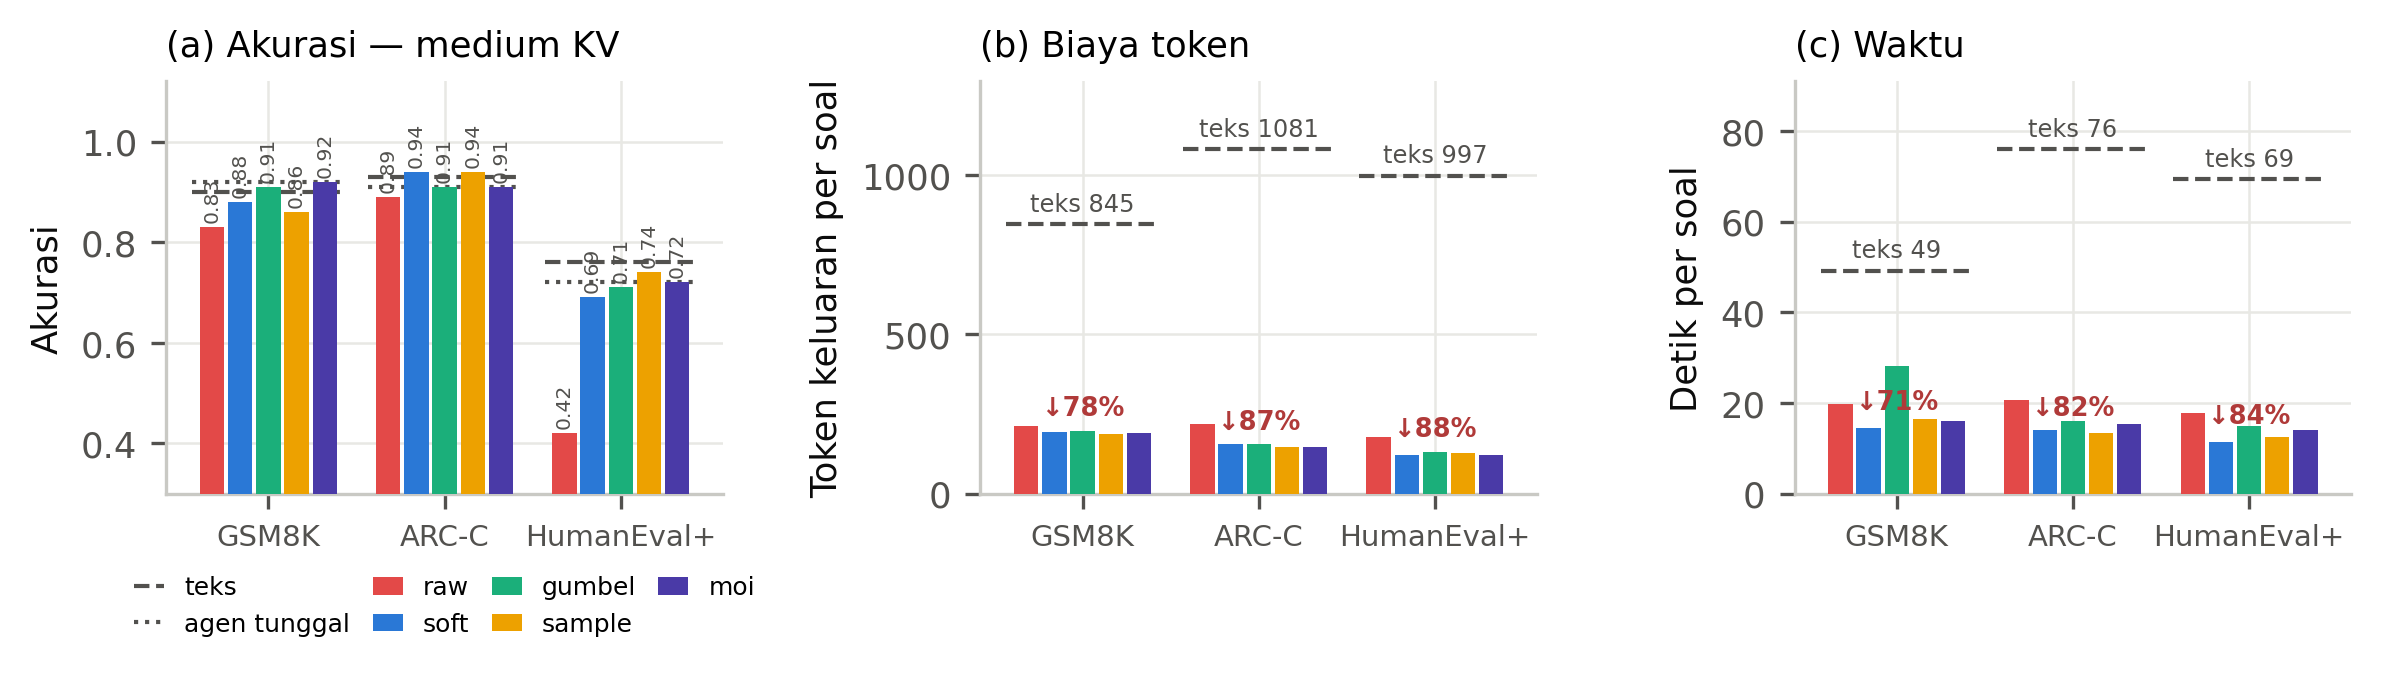
\includegraphics[width=\textwidth]{assets/images/hasil_utama.png}
    \caption{Akurasi, biaya token, dan waktu per soal pada medium KV untuk lima
    persamaan langkah laten. Garis putus-putus menandai medium teks dan garis
    titik-titik menandai agen tunggal.}
    \label{gbr:hasil-utama}
\end{figure}

Pola akurasinya berbeda tajam antar-tugas. Pada GSM8K dan ARC-C ketujuh
perlakuan berada dalam rentang sempit, yaitu 0,83--0,92 dan 0,89--0,94. Pada
HumanEval+ enam perlakuan berada pada 0,69--0,76, sementara persamaan langkah
laten resmi \code{raw} pada medium KV hanya mencapai 0,42.

Setiap pasangan perlakuan dalam satu tugas diuji dengan uji McNemar eksak,
sehingga seluruhnya terdapat 63 pengujian. Delapan pasangan signifikan pada
taraf nominal dan enam bertahan setelah koreksi Holm. Keenamnya berasal dari
HumanEval+ dan seluruhnya melibatkan \code{raw} pada medium KV; tidak ada satu
pun pasangan pada GSM8K maupun ARC-C yang bertahan, dan tidak ada satu pun
pasangan antar-anggota keluarga relaksasi yang bertahan pada tugas mana pun.

\begin{table}[htbp]
\centering
\caption{Seluruh pasangan yang tetap signifikan setelah koreksi Holm atas 63 uji McNemar eksak. Tak satu pun pasangan pada GSM8K dan ARC-C bertahan; seluruh pasangan yang bertahan berasal dari HumanEval+ dan melibatkan \texttt{raw} pada medium KV.}
\label{tab:uji-signifikan}
\small
\begin{tabular}{llrrrr}
\hline
Tugas & Pasangan & $\Delta$ & SK 95\% & $p$ & $p_{\text{Holm}}$ \\
\hline
HumanEval+ & \texttt{raw/kv} vs \texttt{sample/kv} & -0,320 & [-0,42; -0,22] & $1,9\times 10^{-8}$ & $1,2\times 10^{-6}$ \\
HumanEval+ & \texttt{moi/kv} vs \texttt{raw/kv} & +0,300 & [+0,20; +0,40] & $6,9\times 10^{-8}$ & $4,3\times 10^{-6}$ \\
HumanEval+ & \texttt{raw/baseline} vs \texttt{raw/kv} & +0,300 & [+0,20; +0,40] & $2,3\times 10^{-7}$ & $1,4\times 10^{-5}$ \\
HumanEval+ & \texttt{raw/kv} vs \texttt{raw/text} & -0,340 & [-0,45; -0,22] & $3,1\times 10^{-7}$ & $1,9\times 10^{-5}$ \\
HumanEval+ & \texttt{gumbel/kv} vs \texttt{raw/kv} & +0,290 & [+0,19; +0,40] & $1,1\times 10^{-6}$ & $6,4\times 10^{-5}$ \\
HumanEval+ & \texttt{raw/kv} vs \texttt{soft/kv} & -0,270 & [-0,37; -0,17] & $3,5\times 10^{-6}$ & $2,0\times 10^{-4}$ \\
\hline
\end{tabular}
\end{table}


Uji Cochran $Q$ atas kelima persamaan memberikan kesimpulan yang sejalan.
Hipotesis kesamaan kelima persamaan tidak dapat ditolak pada GSM8K
($Q = 7{,}40$; db $= 4$; $p = 0{,}116$) maupun ARC-C ($Q = 6{,}71$; db $= 4$;
$p = 0{,}152$), tetapi ditolak kuat pada HumanEval+ ($Q = 65{,}67$; db $= 4$;
$p < 0{,}0001$).

\section{Keterbedaan Hasil menurut Jenis Tugas}

\begin{figure}[htbp]
    \centering
    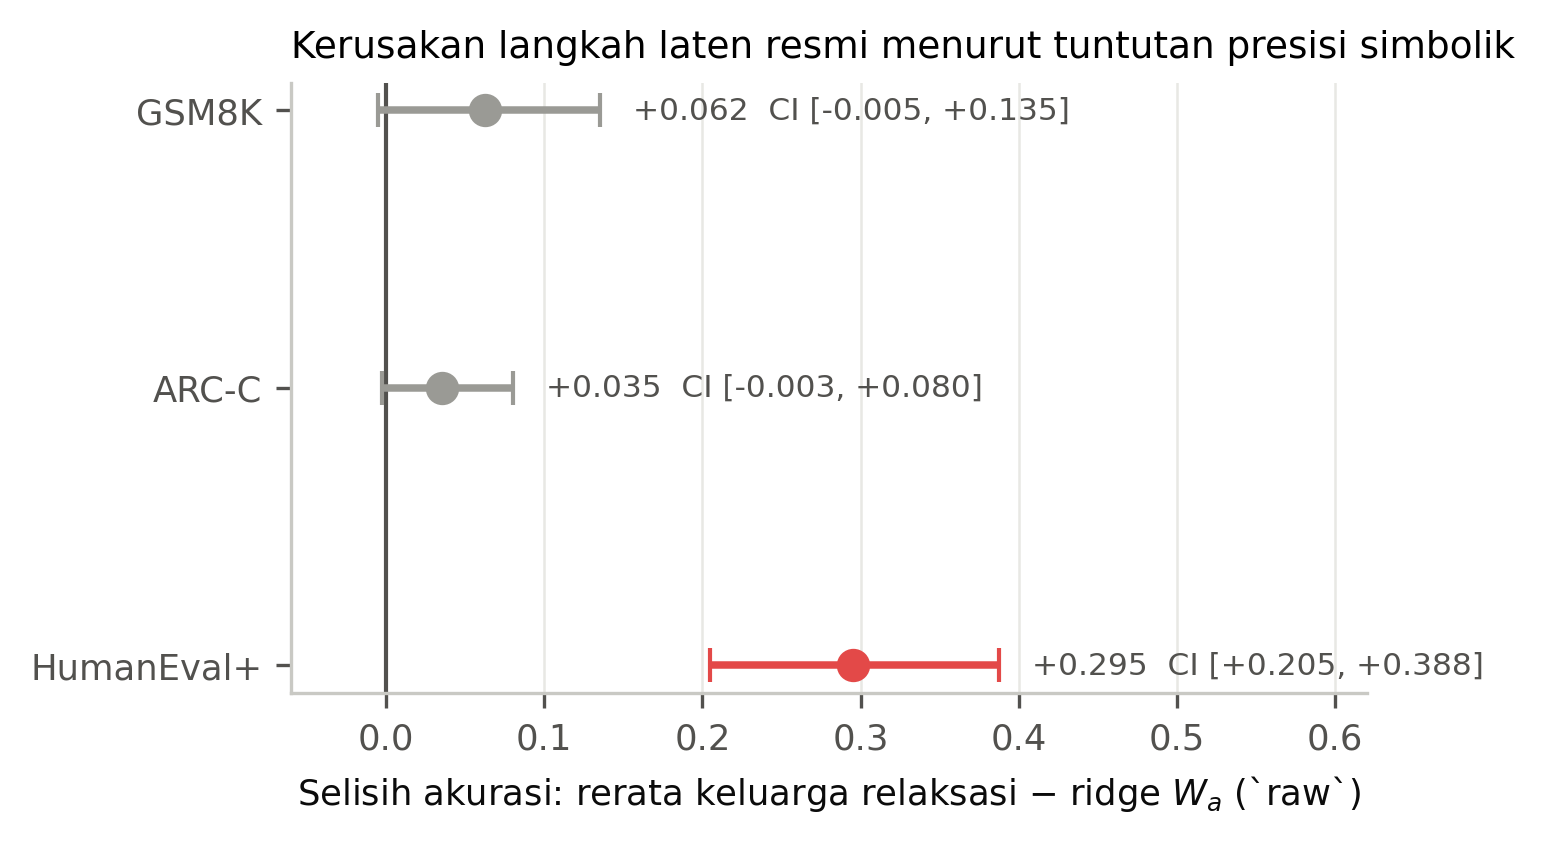
\includegraphics[width=0.85\textwidth]{assets/images/disosiasi.png}
    \caption{Selisih akurasi antara rerata keluarga relaksasi diskret dan ridge
    $W_a$ pada ketiga tugas, dengan selang kepercayaan \textit{bootstrap} 95\%.}
    \label{gbr:disosiasi}
\end{figure}

Selisih akurasi antara rerata keempat anggota keluarga relaksasi dan
\code{raw} adalah $+0{,}062$ pada GSM8K dan $+0{,}035$ pada ARC-C, keduanya
dengan selang kepercayaan yang memuat nol, sedangkan pada HumanEval+ selisihnya
$+0{,}295$ dengan selang kepercayaan $[+0{,}205; +0{,}388]$.

Perbandingan antar-tugas menegaskan keterbedaan tersebut. Kerusakan pada
HumanEval+ berbeda meyakinkan dari kerusakan pada GSM8K ($\Delta\Delta =
+0{,}232$; $p = 0{,}0002$) maupun ARC-C ($\Delta\Delta = +0{,}260$;
$p < 0{,}0001$), sementara GSM8K dan ARC-C tidak dapat dibedakan satu sama lain
($p = 0{,}542$).

Hasil ini mengonfirmasi sebagian hipotesis H2. Bagian yang terkonfirmasi adalah
keterbedaan itu sendiri, yaitu bahwa tugas dengan tuntutan presisi simbolik
tertinggi mengalami kerusakan jauh lebih besar. Bagian yang tidak terkonfirmasi
adalah urutan tiga tingkat yang diramalkan, karena GSM8K dan ARC-C tidak
berbeda satu sama lain; yang didukung data adalah pembedaan dua tingkat.

Satu pembacaan alternatif dapat ditutup di sini. Kerusakan pada HumanEval+ tidak
dapat dinisbahkan kepada medium KV, karena pada tugas yang sama empat perlakuan
lain yang juga memakai medium KV mencapai 0,69--0,74, yaitu setara dengan agen
tunggal (0,72) dan medium teks (0,76). Yang membedakan sel yang runtuh dari
keenam sel lainnya adalah persamaan langkah latennya, bukan mediumnya.

\section{Biaya Komputasi Medium Laten}

\begin{table}[htbp]
\centering
\caption{Efisiensi medium KV relatif terhadap medium teks, per persamaan langkah laten. Penghematan token dihitung atas token keluaran per soal; percepatan atas waktu dinding per soal. Kolom akurasi diulang dari Tabel~\ref{tab:hasil-bench} supaya biaya dan mutu terbaca pada satu baris.}
\label{tab:efisiensi}
\small
\begin{tabular}{llrrr}
\hline
Tugas & Langkah laten & Akurasi & Penghematan token & Percepatan \\
\hline
ARC-C & \texttt{raw} & 0,89 & 79,7\% & $\times3,7$ \\
ARC-C & \texttt{soft} & 0,94 & 85,7\% & $\times5,4$ \\
ARC-C & \texttt{gumbel} & 0,91 & 85,7\% & $\times4,8$ \\
ARC-C & \texttt{sample} & 0,94 & 86,5\% & $\times5,7$ \\
ARC-C & \texttt{moi} & 0,91 & 86,6\% & $\times5,0$ \\
\hline
GSM8K & \texttt{raw} & 0,83 & 75,0\% & $\times2,5$ \\
GSM8K & \texttt{soft} & 0,88 & 77,2\% & $\times3,4$ \\
GSM8K & \texttt{gumbel} & 0,91 & 76,7\% & $\times1,8$ \\
GSM8K & \texttt{sample} & 0,86 & 77,8\% & $\times3,0$ \\
GSM8K & \texttt{moi} & 0,92 & 77,5\% & $\times3,1$ \\
\hline
HumanEval+ & \texttt{raw} & 0,42 & 82,3\% & $\times3,9$ \\
HumanEval+ & \texttt{soft} & 0,69 & 87,8\% & $\times6,1$ \\
HumanEval+ & \texttt{gumbel} & 0,71 & 86,9\% & $\times4,7$ \\
HumanEval+ & \texttt{sample} & 0,74 & 87,4\% & $\times5,6$ \\
HumanEval+ & \texttt{moi} & 0,72 & 87,8\% & $\times4,9$ \\
\hline
\end{tabular}
\end{table}


Tabel~\ref{tab:efisiensi} menunjukkan penghematan token keluaran
75,0\%--87,8\% dan percepatan $\times 1{,}8$--$\times 6{,}1$ terhadap medium
teks. Rentang tersebut memuat rentang 70,8\%--83,7\% yang dilaporkan kerangka
LatentMAS \citep{latentmas}, sehingga klaim efisiensinya terreplikasi pada
implementasi dan perangkat keras yang berbeda.

Mekanisme penghematannya terbaca dari jumlah panggilan model: pada medium teks
setiap soal memicu empat panggilan berkeluaran teks, sedangkan pada medium KV
hanya satu, karena tiga agen perantara menyerahkan pekerjaan lewat
KV-\textit{cache} tanpa memverbalkan penalarannya.

Keunggulan biaya tersebut tidak disertai keunggulan akurasi. Terhadap medium
teks, akurasi sel KV terbaik lebih tinggi pada ARC-C dan GSM8K tetapi lebih
rendah pada HumanEval+, dan tak satu pun selisih tersebut signifikan. Rumusan
yang didukung data adalah kesetaraan akurasi pada biaya yang jauh lebih rendah.

\section{Bukti Mekanisme}

\begin{table}[htbp]
\centering
\caption{Geometri vektor langkah laten pada Qwen3-8B. Kolom terakhir adalah kosinus terhadap baris matriks embedding masukan yang paling dekat; nilai $1$ berarti vektor tepat berimpit dengan embedding sebuah token.}
\label{tab:geometri}
\small
\begin{tabular}{lccc}
\hline
Langkah laten & Bentuk & Anggota ($\star$) & $\max_i \cos(\Phi(h), W_{\text{in}}[i])$ \\
\hline
\texttt{raw} & $\rho\,hM/\lVert hM\rVert$ & tidak & 0,312 [0,16; 0,38] \\
\texttt{soft} & $w = p$ & ya & 0,927 [0,78; 1,00] \\
\texttt{gumbel} & $w = \mathrm{softmax}((\ell+g)/T)$ & ya & 0,985 [0,86; 1,00] \\
\texttt{sample} & $w = e_y$ & ya & 1,000 [1,00; 1,00] \\
\hline
\multicolumn{4}{l}{\footnotesize $\lVert M-I\rVert_F/\lVert I\rVert_F = 1,04$;\quad $\cos(h, hM)$ rerata $= 0,0112$;\quad $\cos(W_{\text{in}}[i], W_{\text{out}}[i])$ rerata $= 0,0041$.} \\
\end{tabular}
\end{table}


Pola di atas sejalan dengan sifat geometris kelima persamaan.
Tabel~\ref{tab:geometri} melaporkan kosinus antara vektor langkah laten dan
baris embedding masukan terdekat: anggota keluarga relaksasi berada pada
0,927--1,000, sedangkan \code{raw} hanya 0,312. Simpangan relatif matriks
realignment terhadap identitas mencapai 1,04 dan kosinus antara \textit{hidden
state} dan hasil pemetaannya hanya 0,0112, sehingga pemetaan tersebut memang
memindahkan vektor jauh dari titik asalnya tanpa mendaratkannya di dekat
embedding token mana pun.

Bukti pendukung berasal dari pengukuran kapasitas kanal yang dilakukan sebelum
lengan \textit{benchmark} dijalankan. Pada kanal laten murni yang membawa nama
fungsi sebagai muatan, persamaan \code{raw} memberikan \textit{recall} 0,000,
sedangkan keempat anggota keluarga relaksasi berada pada 0,34--0,38 dengan
$m=10$. Urutan kerusakan yang kemudian teramati pada lengan \textit{benchmark}
karena itu berstatus ramalan yang diuji, bukan penjelasan yang disusun setelah
melihat angka.

\section{Batas Berlaku Hasil Sementara}

Hasil pada bab ini diperoleh dari satu \textit{backbone} (Qwen3-8B), satu
\textit{seed} per sel, dan subsampel 100 soal per tugas, sehingga ragam
antar-\textit{seed} tidak terukur dan selang kepercayaan yang dilaporkan hanya
mencakup ragam antar-soal. Medium gabungan KV dan teks belum diuji pada ukuran
sampel yang memadai. Urutan tiga tingkat yang diramalkan pada rancangan tidak
terkonfirmasi; yang didukung data adalah pembedaan dua tingkat, yaitu tugas
pembangkitan kode terhadap kedua tugas lainnya. Analisis lengan faktor simbolik
dan pengujian fidelitas simbolik secara rinci disajikan pada laporan akhir.


% ── Daftar Pustaka ──────────────────────────────────────────────────────
% ============================================================================
% DAFTAR PUSTAKA — manual (natbib), urut abjad menurut nama penulis pertama.
% Syarat bimbingan: WAJIB \href ke sumber unduhan; jangan menyitir skripsi S1.
% Penulis paper inti (QuantaAlpha, LatentMAS) sudah dilengkapi dari arXiv.
% Catatan: daftar penulis QuantaAlpha memakai "dkk." (kolaborasi besar);
% cocokkan daftar penuh dengan versi terbit final sebelum sidang.
% ============================================================================
\begin{thebibliography}{99}
\addcontentsline{toc}{chapter}{DAFTAR PUSTAKA}

\bibitem[Ainslie dkk(2023)]{ainslie}
Ainslie, J., Lee-Thorp, J., de Jong, M., Zemlyanskiy, Y., Lebr\'{o}n, F., \&
Sanghai, S. (2023).
\href{https://arxiv.org/abs/2305.13245}{GQA: Training generalized multi-query
transformer models from multi-head checkpoints}. \emph{Proceedings of the 2023
Conference on Empirical Methods in Natural Language Processing (EMNLP)},
4895--4901.

\bibitem[Bain dan Engelhardt(1992)]{bain}
Bain, L. J., \& Engelhardt, M. (1992).
\href{https://archive.org/details/introductiontopr0000bain}{\emph{Introduction
to Probability and Mathematical Statistics}} (2nd ed.). Boston: PWS-KENT.

\bibitem[Chen dkk(2025)]{latentsurvey}
Chen, X., dkk. (2025).
\href{https://arxiv.org/abs/2505.16782}{\emph{Reasoning beyond language: A
comprehensive survey on latent chain-of-thought reasoning}}. arXiv:2505.16782.

\bibitem[Efron dan Tibshirani(1993)]{efron}
Efron, B., \& Tibshirani, R. J. (1993).
\href{https://archive.org/details/introductiontobo0000efro}{\emph{An Introduction
to the Bootstrap}}. New York: Chapman \& Hall.

\bibitem[Fama dan French(2015)]{famafrench}
Fama, E. F., \& French, K. R. (2015).
\href{https://doi.org/10.1016/j.jfineco.2014.10.010}{A five-factor asset pricing
model}. \emph{Journal of Financial Economics}, 116(1), 1--22.

\bibitem[Finin dkk(1994)]{kqml}
Finin, T., Fritzson, R., McKay, D., \& McEntire, R. (1994).
\href{https://doi.org/10.1145/191246.191322}{KQML as an agent communication
language}. \emph{Proceedings of the 3rd International Conference on Information
and Knowledge Management (CIKM)}, 456--463.

\bibitem[Friedman(2001)]{friedman}
Friedman, J. H. (2001).
\href{https://doi.org/10.1214/aos/1013203451}{Greedy function approximation:
A gradient boosting machine}. \emph{The Annals of Statistics}, 29(5),
1189--1232.

\bibitem[Fu dkk(2025)]{cache2cache}
Fu, T., dkk. (2025).
\href{https://arxiv.org/abs/2510.03215}{\emph{Cache-to-Cache: Direct semantic
communication between large language models}}. arXiv:2510.03215.

\bibitem[Goodfellow dkk(2016)]{goodfellow}
Goodfellow, I., Bengio, Y., \& Courville, A. (2016).
\href{https://www.deeplearningbook.org}{\emph{Deep Learning}}.
Cambridge: MIT Press.

\bibitem[Grinold dan Kahn(2000)]{grinold}
Grinold, R. C., \& Kahn, R. N. (2000).
\href{https://archive.org/details/activeportfoliom0000grin}{\emph{Active
Portfolio Management: A Quantitative Approach for Producing Superior Returns
and Controlling Risk}} (2nd ed.). New York: McGraw-Hill.

\bibitem[Guo dkk(2024)]{guo}
Guo, T., Chen, X., Wang, Y., Chang, R., Pei, S., Chawla, N. V., Wiest, O., \&
Zhang, X. (2024).
\href{https://arxiv.org/abs/2402.01680}{\emph{Large language model based
multi-agents: A survey of progress and challenges}}. arXiv:2402.01680.

\bibitem[Han dkk(2026)]{quantaalpha}
Han, J., Zhang, S., Li, W., Dong, Y., Hu, T., dkk. (2026).
\href{https://arxiv.org/abs/2602.07085}{\emph{QuantaAlpha: An Evolutionary
Framework for LLM-Driven Alpha Mining}}. arXiv:2602.07085.

\bibitem[Hao dkk(2024)]{coconut}
Hao, S., Sukhbaatar, S., Su, D., Li, X., Hu, Z., Weston, J., \& Tian, Y. (2024).
\href{https://arxiv.org/abs/2412.06769}{\emph{Training large language models to
reason in a continuous latent space}}. arXiv:2412.06769.

\bibitem[Hoerl dan Kennard(1970)]{ridge}
Hoerl, A. E., \& Kennard, R. W. (1970).
\href{https://doi.org/10.1080/00401706.1970.10488634}{Ridge regression: Biased
estimation for nonorthogonal problems}. \emph{Technometrics}, 12(1), 55--67.

\bibitem[Jensen(1968)]{jensen}
Jensen, M. C. (1968).
\href{https://doi.org/10.1111/j.1540-6261.1968.tb00815.x}{The performance of
mutual funds in the period 1945--1964}. \emph{The Journal of Finance}, 23(2),
389--416.

\bibitem[Johnson dan Wichern(2007)]{johnson}
Johnson, R. A., \& Wichern, D. W. (2007).
\href{https://archive.org/details/appliedmultivari0000john}{\emph{Applied
Multivariate Statistical Analysis}} (6th ed.). Upper Saddle River, NJ: Pearson
Prentice Hall.

\bibitem[Kakushadze(2016)]{kakushadze}
Kakushadze, Z. (2016).
\href{https://arxiv.org/abs/1601.00991}{101 formulaic alphas}.
\emph{Wilmott}, 2016(84), 72--81.

\bibitem[Ke dkk(2017)]{lightgbm}
Ke, G., Meng, Q., Finley, T., Wang, T., Chen, W., Ma, W., Ye, Q., \& Liu, T.-Y.
(2017).
\href{https://papers.nips.cc/paper/6907-lightgbm-a-highly-efficient-gradient-boosting-decision-tree}{LightGBM:
A highly efficient gradient boosting decision tree}. \emph{Advances in Neural
Information Processing Systems}, 30, 3149--3157.

\bibitem[Kingma dan Welling(2014)]{kingma}
Kingma, D. P., \& Welling, M. (2014).
\href{https://arxiv.org/abs/1312.6114}{\emph{Auto-encoding variational Bayes}}.
\emph{Proceedings of the 2nd International Conference on Learning
Representations (ICLR)}. arXiv:1312.6114.

\bibitem[Li dkk(2025)]{rdagent}
Li, Y., Yang, X., Yang, X., Xu, M., Wang, X., Liu, W., \& Bian, J. (2025).
\href{https://arxiv.org/abs/2505.15155}{\emph{R\&D-Agent-Quant: A multi-agent
framework for data-centric factors and model joint optimization}}.
arXiv:2505.15155.

\bibitem[Markowitz(1952)]{markowitz}
Markowitz, H. (1952).
\href{https://doi.org/10.1111/j.1540-6261.1952.tb01525.x}{Portfolio selection}.
\emph{The Journal of Finance}, 7(1), 77--91.

\bibitem[Zhuang dkk(2025)]{moi}
Zhuang, Y., Liu, S., Cheng, S., Zhang, Y., Wang, X., \& Zhang, C. (2025).
\href{https://arxiv.org/abs/2505.14827}{\emph{Mixture of inputs: Text
generation beyond discrete token sampling}}. arXiv:2505.14827. Dipresentasikan
pada \emph{Advances in Neural Information Processing Systems} (NeurIPS 2025).

\bibitem[Mikolov dkk(2013)]{mikolov2013}
Mikolov, T., Chen, K., Corrado, G., \& Dean, J. (2013).
\href{https://arxiv.org/abs/1301.3781}{\emph{Efficient estimation of word
representations in vector space}}. arXiv:1301.3781.

\bibitem[Park dkk(2024)]{lrh}
Park, K., Choe, Y. J., \& Veitch, V. (2024).
\href{https://arxiv.org/abs/2311.03658}{\emph{The linear representation hypothesis
and the geometry of large language models}}. Proceedings of the 41st International
Conference on Machine Learning (ICML). arXiv:2311.03658.

\bibitem[Russell dan Norvig(2021)]{russellnorvig}
Russell, S., \& Norvig, P. (2021).
\href{https://archive.org/details/artificialintell0000russ_v4h1}{\emph{Artificial
Intelligence: A Modern Approach}} (4th ed.). Hoboken, NJ: Pearson.

\bibitem[Sharpe(1964)]{capm}
Sharpe, W. F. (1964).
\href{https://doi.org/10.1111/j.1540-6261.1964.tb02865.x}{Capital asset prices:
A theory of market equilibrium under conditions of risk}. \emph{The Journal of
Finance}, 19(3), 425--442.

\bibitem[Sharpe(1994)]{sharpe}
Sharpe, W. F. (1994).
\href{https://doi.org/10.3905/jpm.1994.409501}{The Sharpe ratio}.
\emph{The Journal of Portfolio Management}, 21(1), 49--58.

\bibitem[Spearman(1904a)]{spearman}
Spearman, C. (1904a).
\href{https://doi.org/10.2307/1412159}{The proof and measurement of
association between two things}. \emph{The American Journal of Psychology},
15(1), 72--101.

\bibitem[Spearman(1904b)]{spearmanfactor}
Spearman, C. (1904b).
\href{https://doi.org/10.2307/1412107}{``General intelligence,'' objectively
determined and measured}. \emph{The American Journal of Psychology}, 15(2),
201--292.

\bibitem[Su dkk(2024)]{roformer}
Su, J., Ahmed, M., Lu, Y., Pan, S., Bo, W., \& Liu, Y. (2024).
\href{https://arxiv.org/abs/2104.09864}{RoFormer: Enhanced transformer with
rotary position embedding}. \emph{Neurocomputing}, 568, 127063.

% Buku cetak berbahasa Indonesia; tak ada unduhan bebas legal — tautan ke katalog
% perpustakaan (OpenLibrary Telkom). Cocokkan/ganti bila punya sumber lain.
\bibitem[Tandelilin(2010)]{tandelilin}
Tandelilin, E. (2010).
\href{https://openlibrary.telkomuniversity.ac.id/pustaka/155750/portofolio-dan-investasi-teori-dan-aplikasi.html}{\emph{Portofolio
dan Investasi: Teori dan Aplikasi}} (Edisi Pertama). Yogyakarta: Kanisius.

\bibitem[Tang dkk(2025)]{alphaagent}
Tang, Z., Chen, Z., Yang, J., Mai, J., Zheng, Y., Wang, K., Chen, J., \& Lin, L.
(2025).
\href{https://arxiv.org/abs/2502.16789}{\emph{AlphaAgent: LLM-driven alpha
mining with regularized exploration to counteract alpha decay}}.
arXiv:2502.16789.

\bibitem[Vaswani dkk(2017)]{vaswani}
Vaswani, A., Shazeer, N., Parmar, N., Uszkoreit, J., Jones, L., Gomez, A. N.,
Kaiser, L., \& Polosukhin, I. (2017).
\href{https://arxiv.org/abs/1706.03762}{\emph{Attention is all you need}}.
\emph{Advances in Neural Information Processing Systems}, 30.

\bibitem[Wooldridge dan Jennings(1995)]{wooldridge}
Wooldridge, M., \& Jennings, N. R. (1995).
\href{https://doi.org/10.1017/S0269888900008122}{Intelligent agents: Theory and
practice}. \emph{The Knowledge Engineering Review}, 10(2), 115--152.

\bibitem[Wooldridge(2009)]{wooldridge2009}
Wooldridge, M. (2009).
\href{https://archive.org/details/introductiontomu0000wool}{\emph{An
Introduction to MultiAgent Systems}} (2nd ed.). Chichester: Wiley.

\bibitem[Yang dkk(2020)]{qlib}
Yang, X., Liu, W., Zhou, D., Bian, J., \& Liu, T.-Y. (2020).
\href{https://arxiv.org/abs/2009.11189}{\emph{Qlib: An AI-oriented quantitative
investment platform}}. arXiv:2009.11189.

\bibitem[Yang dkk(2025)]{qwen3}
Yang, A., dkk. (Qwen Team). (2025).
\href{https://arxiv.org/abs/2505.09388}{\emph{Qwen3 technical report}}.
arXiv:2505.09388.

\bibitem[Yu dkk(2023)]{alphagen}
Yu, S., Xue, H., Ao, X., Pan, F., He, J., Tu, D., \& He, Q. (2023).
\href{https://arxiv.org/abs/2306.12964}{Generating synergistic formulaic alpha
collections via reinforcement learning}. \emph{Proceedings of the 29th ACM
SIGKDD Conference on Knowledge Discovery and Data Mining} (KDD '23).

\bibitem[Zhang dkk(2025)]{softthinking}
Zhang, Z., He, X., Yan, W., Shen, A., Zhao, C., Wang, S., Shen, Y., \& Wang,
X. E. (2025).
\href{https://arxiv.org/abs/2505.15778}{\emph{Soft thinking: Unlocking the
reasoning potential of LLMs in continuous concept space}}. arXiv:2505.15778.

\bibitem[Zou dkk(2025)]{latentmas}
Zou, J., Qiu, R., Li, G., Yang, X., Tieu, K., Lu, P., Shen, K., Tong, H.,
Choi, Y., He, J., Zou, J., Wang, M., \& Yang, L. (2025).
\href{https://arxiv.org/abs/2511.20639}{\emph{Latent collaboration in multi-agent
systems}}. arXiv:2511.20639.

\end{thebibliography}


% ── Lampiran ────────────────────────────────────────────────────────────
\appendix
\chapter{Tabel Lengkap Sel Lengan \textit{Benchmark}}
\label{lamp:sel-bench}

Seluruh 21 sel utama lengan \textit{benchmark}. Kolom \textit{format} adalah proporsi keluaran berbentuk sah; kolom CJK adalah cacah jawaban yang memuat aksara Tionghoa pada tugas berbahasa Inggris.

\begin{longtable}{llrrrrrr}
\hline
Tugas & Sel & $n$ & Akurasi & SK 95\% & Format & Token/soal & CJK \\
\hline\endhead
GSM8K & \texttt{gumbel/kv} & 100 & 0,91 & [0,85; 0,96] & 1,00 & 197 & 0 \\
GSM8K & \texttt{moi/kv} & 100 & 0,92 & [0,86; 0,97] & 1,00 & 190 & 1 \\
GSM8K & \texttt{raw/baseline} & 100 & 0,92 & [0,86; 0,97] & 1,00 & --- & --- \\
GSM8K & \texttt{raw/kv} & 100 & 0,83 & [0,75; 0,90] & 0,98 & 212 & 2 \\
GSM8K & \texttt{raw/text} & 100 & 0,90 & [0,84; 0,95] & 1,00 & 845 & 0 \\
GSM8K & \texttt{sample/kv} & 100 & 0,86 & [0,79; 0,92] & 0,97 & 187 & 0 \\
GSM8K & \texttt{soft/kv} & 100 & 0,88 & [0,81; 0,94] & 1,00 & 192 & 0 \\
\hline
ARC-C & \texttt{gumbel/kv} & 100 & 0,91 & [0,85; 0,96] & 0,98 & 154 & 1 \\
ARC-C & \texttt{moi/kv} & 100 & 0,91 & [0,85; 0,96] & 0,98 & 145 & 0 \\
ARC-C & \texttt{raw/baseline} & 100 & 0,91 & [0,85; 0,96] & 1,00 & 271 & 0 \\
ARC-C & \texttt{raw/kv} & 100 & 0,89 & [0,83; 0,95] & 1,00 & 219 & 3 \\
ARC-C & \texttt{raw/text} & 100 & 0,93 & [0,88; 0,98] & 1,00 & 1081 & 0 \\
ARC-C & \texttt{sample/kv} & 100 & 0,94 & [0,89; 0,98] & 1,00 & 146 & 0 \\
ARC-C & \texttt{soft/kv} & 100 & 0,94 & [0,89; 0,98] & 1,00 & 154 & 1 \\
\hline
HumanEval+ & \texttt{gumbel/kv} & 100 & 0,71 & [0,62; 0,80] & 0,97 & 131 & 0 \\
HumanEval+ & \texttt{moi/kv} & 100 & 0,72 & [0,63; 0,81] & 1,00 & 122 & 0 \\
HumanEval+ & \texttt{raw/baseline} & 100 & 0,72 & [0,63; 0,80] & 1,00 & 122 & 0 \\
HumanEval+ & \texttt{raw/kv} & 100 & 0,42 & [0,32; 0,52] & 1,00 & 177 & 1 \\
HumanEval+ & \texttt{raw/text} & 100 & 0,76 & [0,68; 0,84] & 1,00 & 997 & 0 \\
HumanEval+ & \texttt{sample/kv} & 100 & 0,74 & [0,65; 0,82] & 1,00 & 126 & 0 \\
HumanEval+ & \texttt{soft/kv} & 100 & 0,69 & [0,60; 0,78] & 0,96 & 122 & 0 \\
\hline
\end{longtable}

\chapter{Transkrip Rantai Agen}
\label{lamp:transkrip}

Keluaran verbatim keempat agen untuk satu soal GSM8K yang sama, dibandingkan antara persamaan langkah laten resmi (\texttt{raw}) dan salah satu anggota keluarga relaksasi diskret (\texttt{gumbel}), pada medium gabungan KV dan teks. Teks tidak disunting; pemenggalan baris ditambahkan agar muat di halaman.

\section*{Persamaan langkah laten \texttt{raw}}
\subsection*{Agen \texttt{planner}}
\begin{lstlisting}[basicstyle=\ttfamily\scriptsize,breaklines=true,frame=single]
- **Understand the problem**: Identify that Mandy owes $100 with a monthly interest rate of 2%, and she pays after 3 months.  
- **Calculate the total interest**: Use the formula for simple interest: Interest = Principal [U+00D7] Rate [U+00D7] Time.  
- **Add the interest to the principal**: Calculate the total amount owed by adding the interest to the original $100.  
- **Determine the final payment**: Present the total amount Mandy should pay Benedict after 3 months.
\end{lstlisting}

\subsection*{Agen \texttt{critic}}
\begin{lstlisting}[basicstyle=\ttfamily\scriptsize,breaklines=true,frame=single]
Original Plan:  
- **Understand the problem**: Identify that Mandy owes $100 with a monthly interest rate of 2%, and she pays after 3 months.  
- **Calculate the total interest**: Use the formula for simple interest: Interest = Principal [U+00D7] Rate [U+00D7] Time.  
- **Add the interest to the principal**: Calculate the total amount owed by adding the interest to the original $100.  
- **Determine the final payment**: Present the total amount Mandy should pay Benedict after 3 months.

Feedback:  
The original plan is clear and logically structured, but it can be slightly refined for better precision. Specifically, the step "Use the formula for simple interest" should include the exact formula (Interest = Principal [U+00D7] Rate [U+00D7] Time) to ensure clarity. Additionally, the step "Add the interest to the principal" could be more explicitly worded as "Calculate the total amount by adding the calculated interest to the principal amount." These small adjustments will make the plan even more precise and easier to follow.
\end{lstlisting}

\subsection*{Agen \texttt{refiner}}
\begin{lstlisting}[basicstyle=\ttfamily\scriptsize,breaklines=true,frame=single]
Refined Plan:  
- **Understand the problem**: Identify that Mandy owes $100 with a monthly interest rate of 2%, and she pays after 3 months.  
- **Calculate the total interest**: Use the simple interest formula: Interest = Principal [U+00D7] Rate [U+00D7] Time, where Principal = $100, Rate = 2% (or 0.02), and Time = 3 months.  
- **Compute the total amount owed**: Add the calculated interest to the original principal amount of $100.  
- **Determine the final payment**: Present the total amount Mandy should pay Benedict after 3 months, including both the principal and the accumulated interest.
\end{lstlisting}

\subsection*{Agen \texttt{judger}}
\begin{lstlisting}[basicstyle=\ttfamily\scriptsize,breaklines=true,frame=single]
To solve the problem, we need to calculate the total amount Mandy should pay Benedict after 3 monthss, including both the principal and the accumulated interest.

### Step-by-step Reasoning:

1. **Identify the principal amount**:  
   - The principal amount is $100.

2. **Determine the monthly interest rate**:  
   - The monthly interest.rate is 2%, which can be expressed as a decimal: 0.02.

3. **Calculate the total interest over 3 monthss**:  
   - Use the simple interest formula:  
     $$
     \text{Interest} = \text{Principal} \times \text{Rate} \times \text{Time}
     $$
     $$
     \text{Interest} = 100 \times 0.02 \times 3 = 6
     $$

4. **Add the interest to the principal to get the total amount owed**:  
   - Total amount = Principal + Interest  
     $$
     \text{Total Amount} = 100 + 6 = 106
     $$

### Final Answer:
$$
\boxed{106}
$$
\end{lstlisting}

\section*{Persamaan langkah laten \texttt{gumbel}}
\subsection*{Agen \texttt{planner}}
\begin{lstlisting}[basicstyle=\ttfamily\scriptsize,breaklines=true,frame=single]
- Calculate the monthly interest for the first month by multiplying the principal amount ($100) by the monthly interest rate (2%).  
- Add the first month's interest to the principal to get the new balance after the first month.  
- Calculate the monthly interest for the second month using the updated balance.  
- Add the second month's interest to the balance to get the new balance after the second month.  
- Calculate the monthly interest for the third month using the updated balance after two months.  
- Add the third month's interest to the balance to determine the total amount Mandy should pay Benedict after three months.
\end{lstlisting}

\subsection*{Agen \texttt{critic}}
\begin{lstlisting}[basicstyle=\ttfamily\scriptsize,breaklines=true,frame=single]
Feedback:  
The original plan is incomplete and lacks clarity in the steps. It should explicitly mention that the interest is compounded monthly, which means each month's interest is calculated based on the current balance (including previously accrued interest). The plan should also include a clear instruction to calculate the total amount after three months by summing up the principal and all the compounded interest. Additionally, it would be helpful to specify that the final amount includes both the original debt and the accumulated interest over the three months.
\end{lstlisting}

\subsection*{Agen \texttt{refiner}}
\begin{lstlisting}[basicstyle=\ttfamily\scriptsize,breaklines=true,frame=single]
- Start with the principal amount of $100.  
- Calculate the monthly interest for each of the three months using the formula: Interest = Principal [U+00D7] Monthly Interest Rate (2%).  
- Add the first month's interest to the principal to get the new balance after the first month.  
- Use the updated balance as the new principal for the second month and calculate the interest again.  
- Add the second month's interest to the balance to get the new balance after the second month.  
- Use the updated balance as the new principal for the third month and calculate the interest again.  
- Add the third month's interest to the balance to determine the total amount Mandy should pay Benedict after three months.
\end{lstlisting}

\subsection*{Agen \texttt{judger}}
\begin{lstlisting}[basicstyle=\ttfamily\scriptsize,breaklines=true,frame=single]
To solve the problem, we need to calculate the total amount Mandy should pay Benedict after 3 months, including monthly compound interest.

### Step-by-Step Calculation:

1. **Initial Principal**: $100  
2. **Monthly Interest Rate**: 2% = 0.02  
3. **Time Period**: 3 months  

We use the formula for compound interest:  
$$
A = P(1 + r)^t
$$  
Where:  
- $ A $ is the final amount  
- $ P $ is the principal ($100)  
- $ r $ is the monthly interest rate (0.02)  
- $ t $ is the time in months (3)

$$
A = 100(1 + 0.02)^3 = 100(1.02)^3
$$

Calculate $ (1.02)^3 $:  
$$
(1.02)^3 = 1.061208
$$

Now multiply by the principal:  
$$
A = 100 \times 1.061208 = 106.1208
$$

Rounded to two decimal places:  
$$
\boxed{106.12}
$$
\end{lstlisting}

\section*{Contoh Korupsi Token yang Terekam}

Cuplikan jawaban yang memuat aksara di luar ASCII pada tugas berbahasa Inggris. Aksara tersebut ditampilkan sebagai titik kode Unicode.

\begin{longtable}{lp{8cm}}
\hline
Sel & Cuplikan \\
\hline\endhead
\texttt{arc\_challenge\_gumbel\_kv\_s0} & \texttt{of ice, which scrapes and[U+78E8][U+5E73] (} \\
\texttt{arc\_challenge\_raw\_kv\_s0} & \texttt{the effects of a hypoxic[U+4E8B][U+4EF6].} \\
\texttt{arc\_challenge\_soft\_kv\_s0} & \texttt{[U+73CA][U+745A][U+7901][U+662F]} \\
\texttt{gsm8k\_moi\_kv\_s0} & \texttt{1. **[U+786E][U+5B9A][U+6BCF][U+79CD]} \\
\texttt{gsm8k\_raw\_kv\_s0} & \texttt{To solve the problem of[U+30B3]  O} \\
\texttt{humanevalplus\_raw\_kv\_s0} & \texttt{'No'     \#Count.digits.in[U+6574][U+4E2A]fi} \\
\hline
\end{longtable}

\chapter{Hiperparameter dan Lingkungan Eksekusi}
\label{lamp:hparam}

\begin{longtable}{ll}
\hline
Parameter & Nilai \\
\hline\endhead
Model & \texttt{Qwen/Qwen3-8B} \\
Ukuran kosakata $V$ & 151.936 \\
Dimensi \textit{hidden} $d$ & 4096 \\
Embedding terikat & tidak \\
Langkah laten $m$ & 10 \\
Suhu langkah laten $T$ & 0,70 \\
Regularisasi ridge $\lambda$ & $10^{-5}$ \\
Parameter MoI $\beta$ & 1 \\
Suhu pembangkitan & 0,60 \\
\textit{top-p} & 0,95 \\
Token baru maksimum & 2048 \\
Rantai agen & \texttt{planner}, \texttt{critic}, \texttt{refiner}, \texttt{judger} \\
Subsampel per sel & 100 \\
\textit{Seed} pengambilan sampel & 0 \\
\textit{Seed} pembangkitan & 0 \\
GPU & NVIDIA A40 46 GB, CUDA 12.8 \\
Kerangka kerja & PyTorch 2.6.0+cu124, HuggingFace Transformers \\
\hline
\end{longtable}


\end{document}
